\documentclass[uplatex]{jsarticle}
\usepackage[dvipdfmx]{graphicx}
\usepackage{listings}
\usepackage{url}
\title{マイコン講習マニュアル}
\date{\empty}
\author{京都大学機械研究会 \\ 工学部情報学科 \\ 松本直樹}

\begin{document}
\maketitle
\section{はじめに}
マイコンとは、いわゆるマイクロコンピューターの略称であり(諸説あり)、
冷蔵庫や洗濯機などありとあらゆる電気製品に組み込まれているコンピュータである。

京大機械研究会ではArduinoを利用してロボットの制御を行っている。
今回の講習ではArudinoの基本的な利用方法とプログラミングの基本を会得することを目的としている。

\section{Arduinoとは?}
ArduinoとはAVRマイコンを利用した、組み込みマイコンのシステムの一種である。
ArduinoではArduino IDEなる開発環境を無償で利用することができ、
C/C++ライクな開発言語で開発することが出来る。
従来のPICやAVRとは大きく異なり、Arduinoというプラットフォーム形態を確立しているため、
抽象度の高いプログラミングが可能であり、初心者にとっては非常に扱いやすいシステムである。

Arduinoで利用可能な機能としては、A/D変換、PWM、I2C、SPIなど、機械研において制作するロボットに
に必要な機能はほぼ網羅している。

\section{機械研マイコンボード}
今回の講習で利用するボードは、回路講習で作った機械研マイコンボードである。
このマイコンボードは部内ロボコンだけでなく、合同ロボコンやNFでの展示物にも利用できるため、
是非使い方を習得し、製作の役に立ててもらいたい。
\subsection{回路図}
機械研マイコンボードの回路図は以下のとおりである。
\begin{figure}
    \centering
    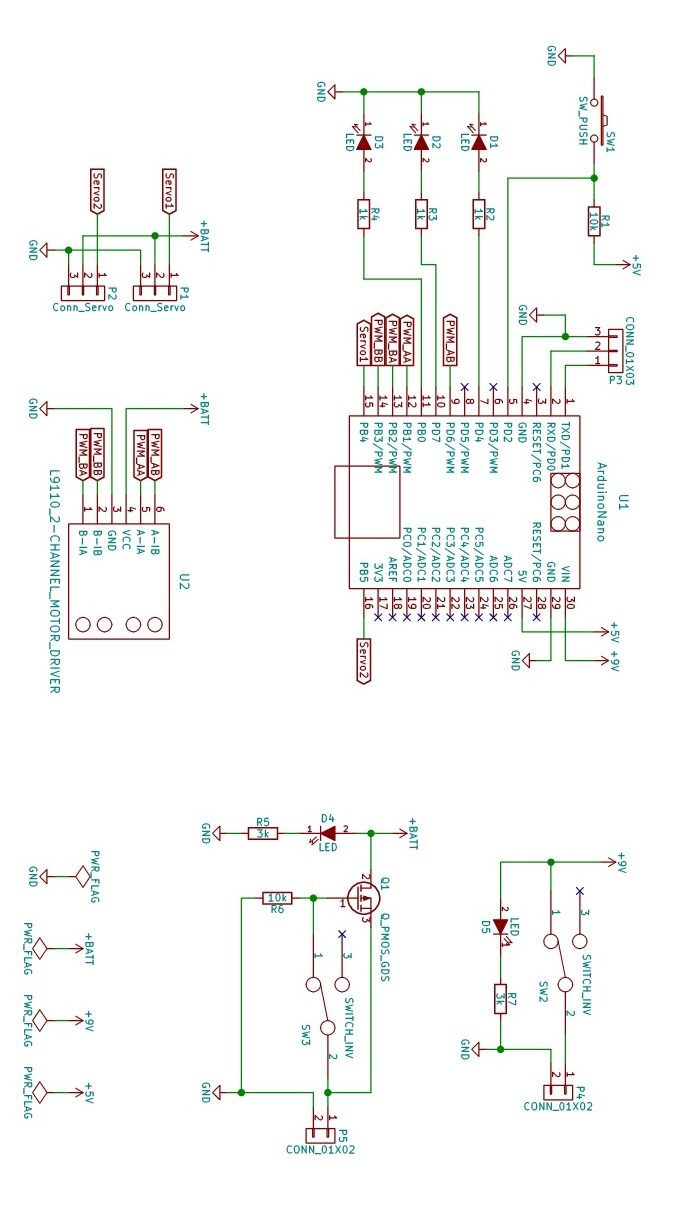
\includegraphics[width=10cm]{circuit.jpg}
    \caption{機械研マイコンボード回路図}
\end{figure}
\subsection{実体配線図}
機械研マイコンボードの実体配線図は以下のとおりである。
\begin{figure}
    \centering
    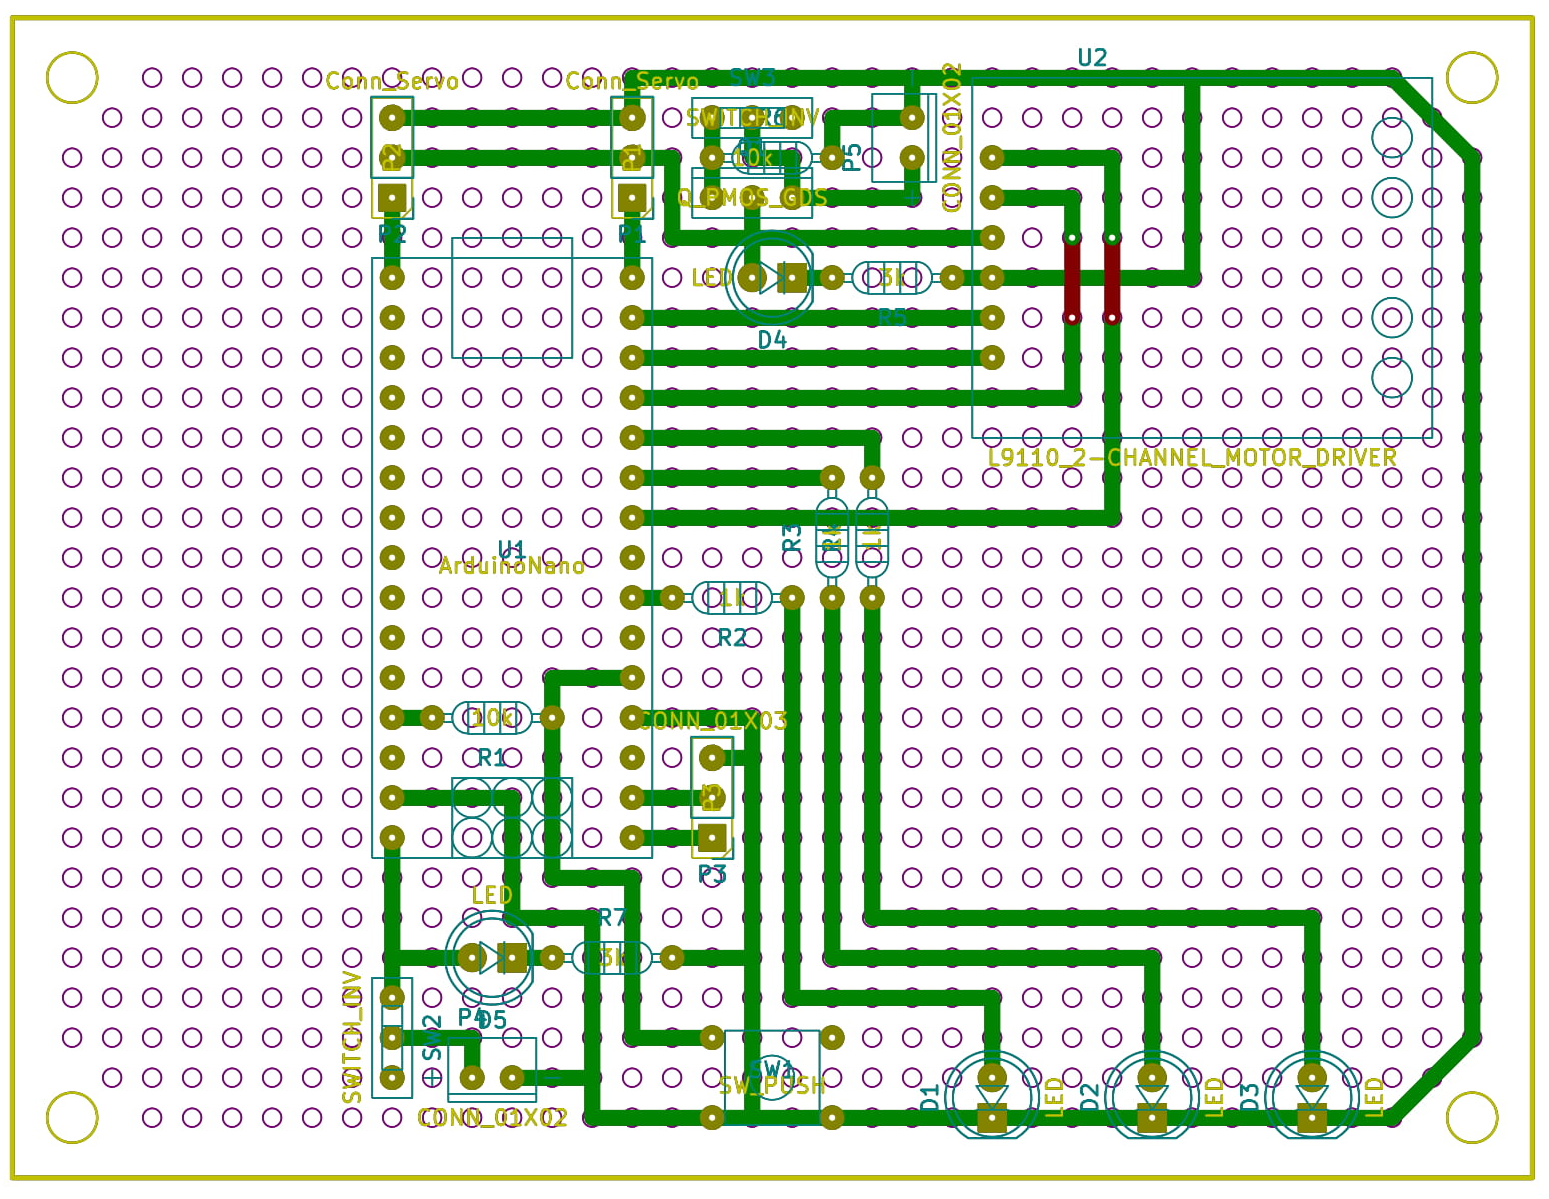
\includegraphics[width=15cm]{wiring.png}
    \caption{機械研マイコンボード実体配線図}
\end{figure}
\subsection{利用可能な機能}
Arduino nanoにおいて利用可能な機能は以下のとおりである。
\begin{itemize}
    \item デジタルI/Oピン 14本
    \item PWM 6本
    \item アナログ入力ピン 8本(AD変換精度 10bit)
    \item タイマー3つ(8bit 2つ・16bit 1つ)
    \item I2C 1つ
    \item SPI 1つ
    \item UART 1つ
\end{itemize}
タイマーはPWMと競合するため、同時に利用する際は注意が必要である。
また、I2CやSPI、UARTもデジタルI/Oピン、アナログ入力ピンと重複しているため、
同時に使えるピンに気をつける必要がある。

以下にArduino nanoにおけるピンの機能割当の図を示す。

\begin{figure}[htbp]
    \centering
     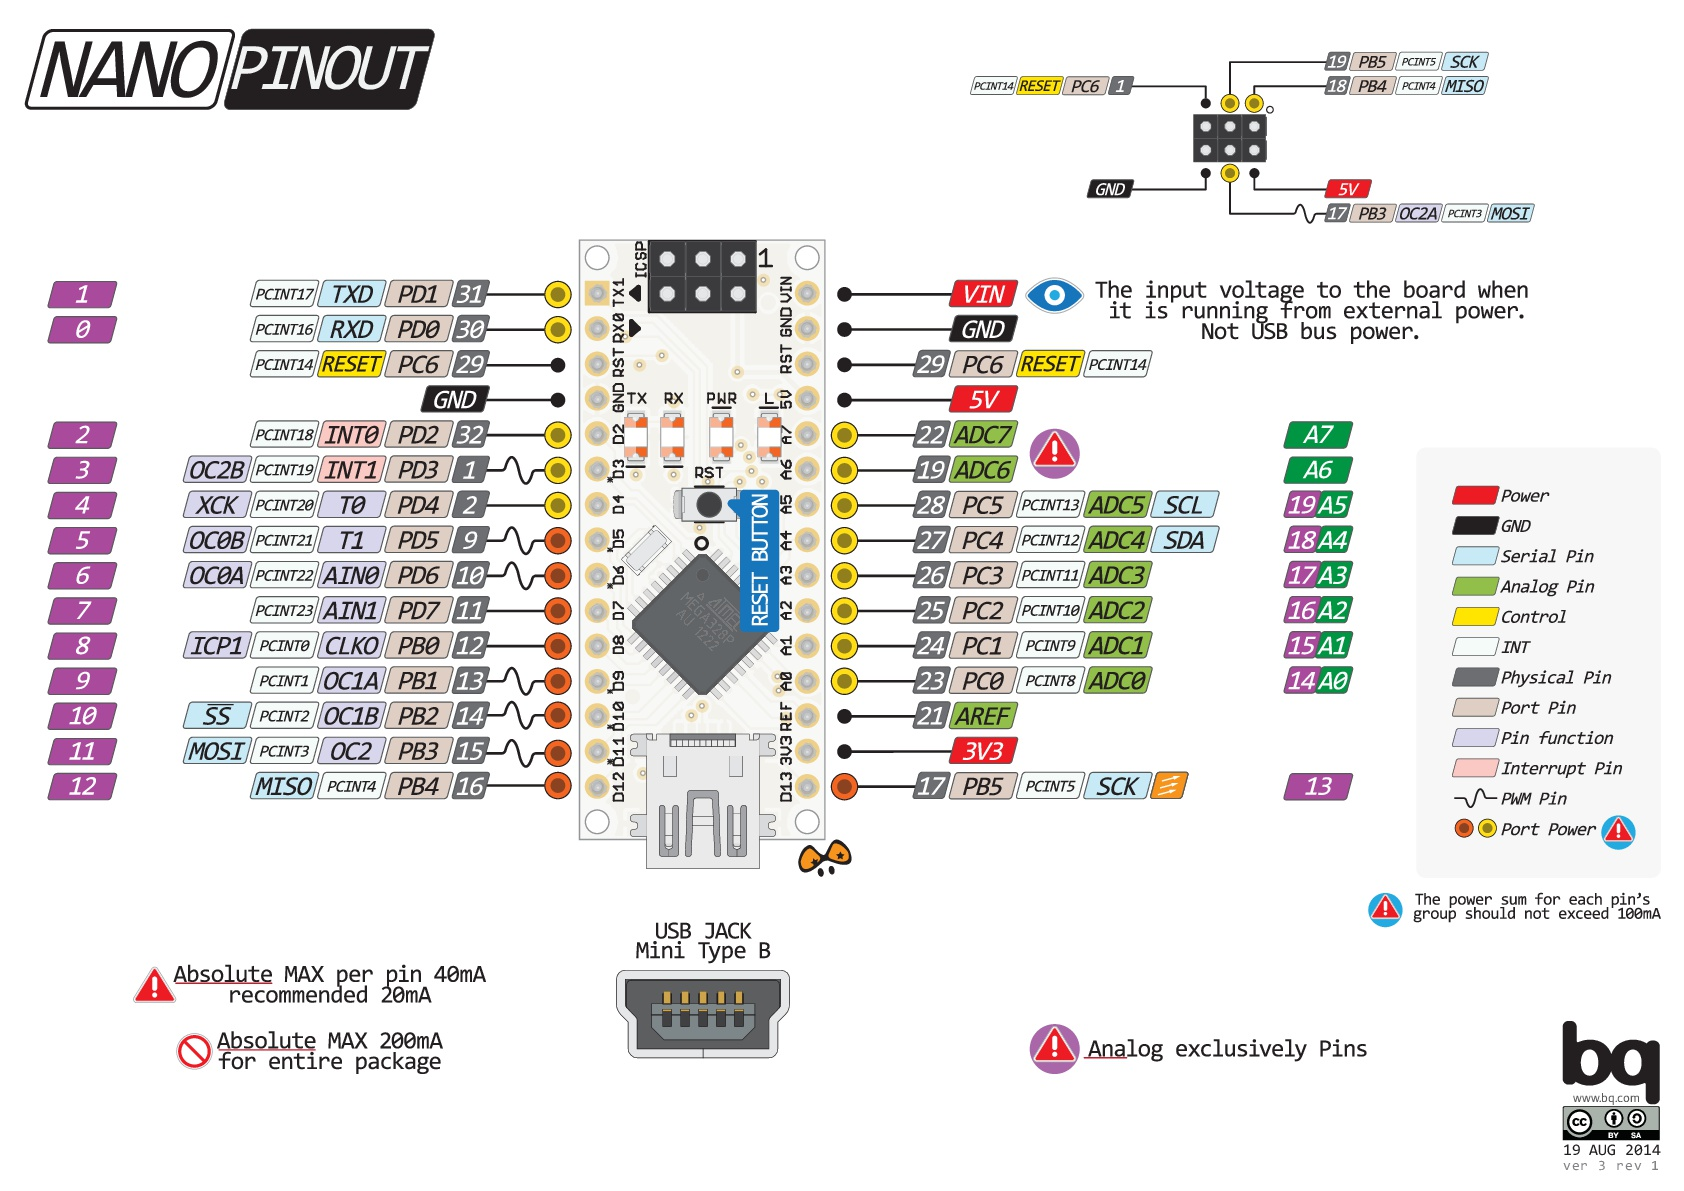
\includegraphics[width=15cm]{nano.jpg}
    \caption{Arduino nanoにおけるピンの機能割当}
\end{figure}

\section{開発環境の構築}
手元のPC上にArduinoの開発環境を構築する。
\subsection{ドライバのインストール}
機械研マイコンボードでは純正Arduinoとは異なり、ドライバを別途インストールする必要がある。
ドライバを以下の手順でインストールする。

1.「CH340 ドライバ」と検索する。検索結果から「CH340 Drivers for Windows,Mac and Linux」
を選択する。
\begin{figure}[htbp]
    \centering
     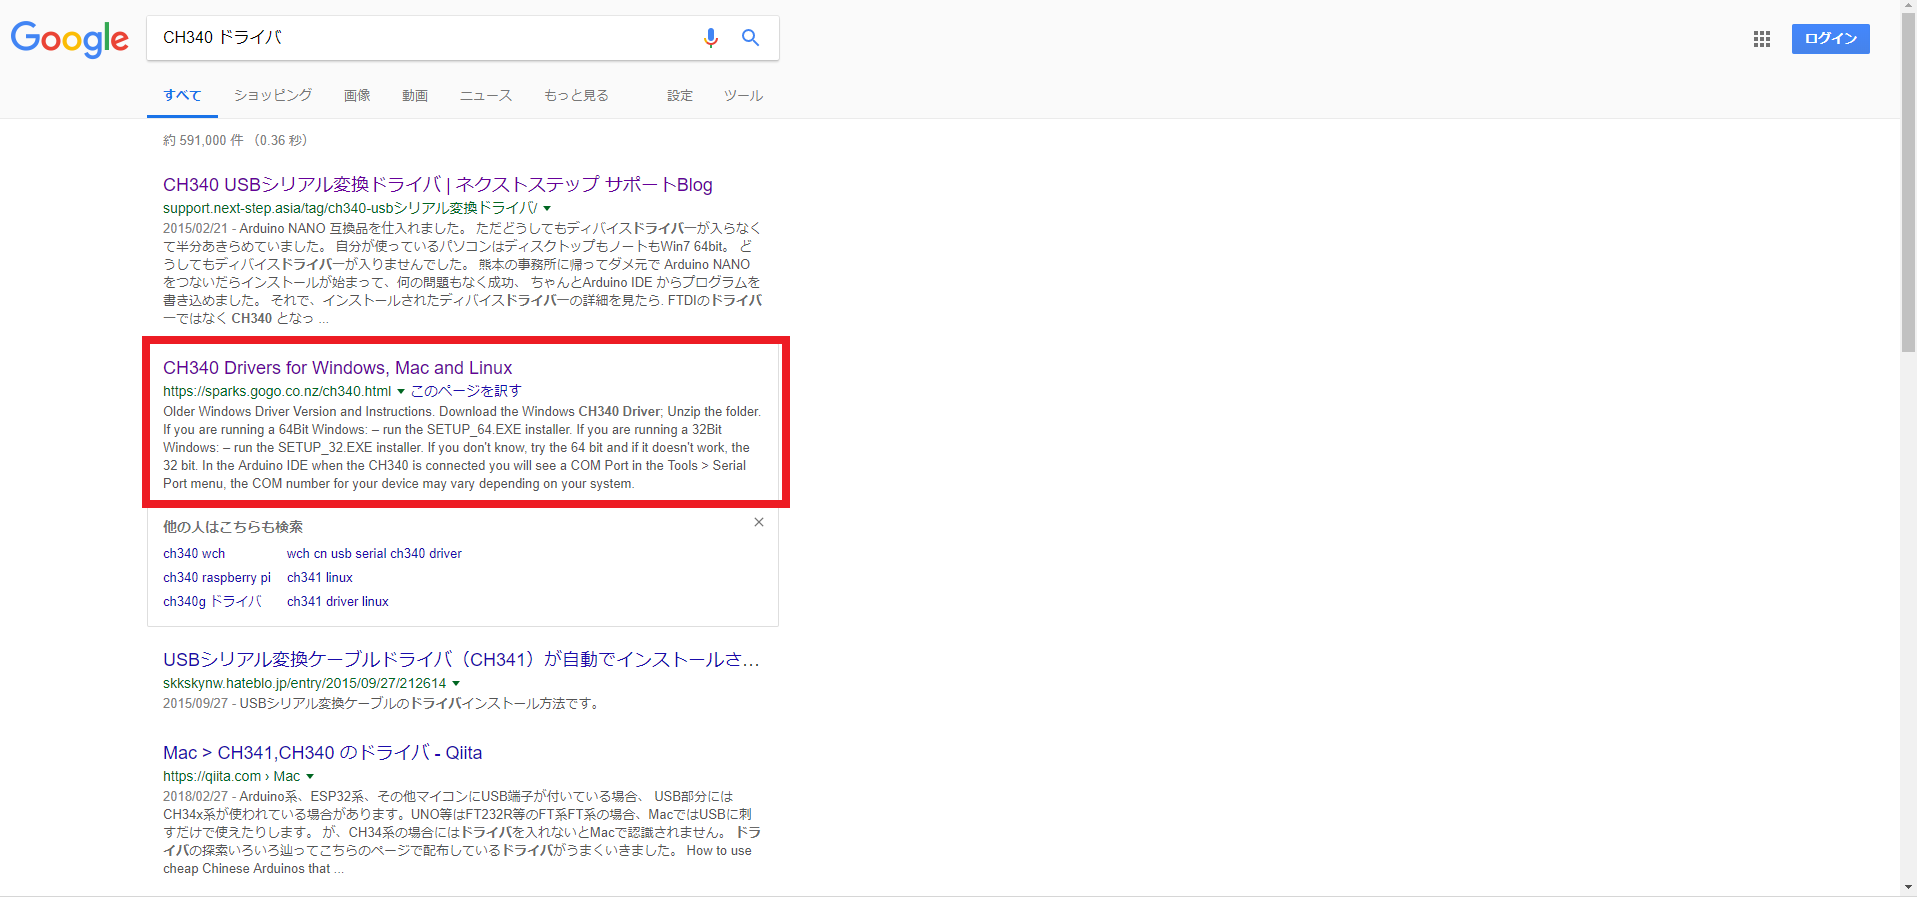
\includegraphics[width=13cm]{driver_1.png}
    \caption{「CH340 ドライバ」と検索する}
\end{figure}

2.Windowsの項目から「Windows CH340 Driver」を選択する。
すると、ドライバファイルがダウンロードされる。
\begin{figure}
    \centering
    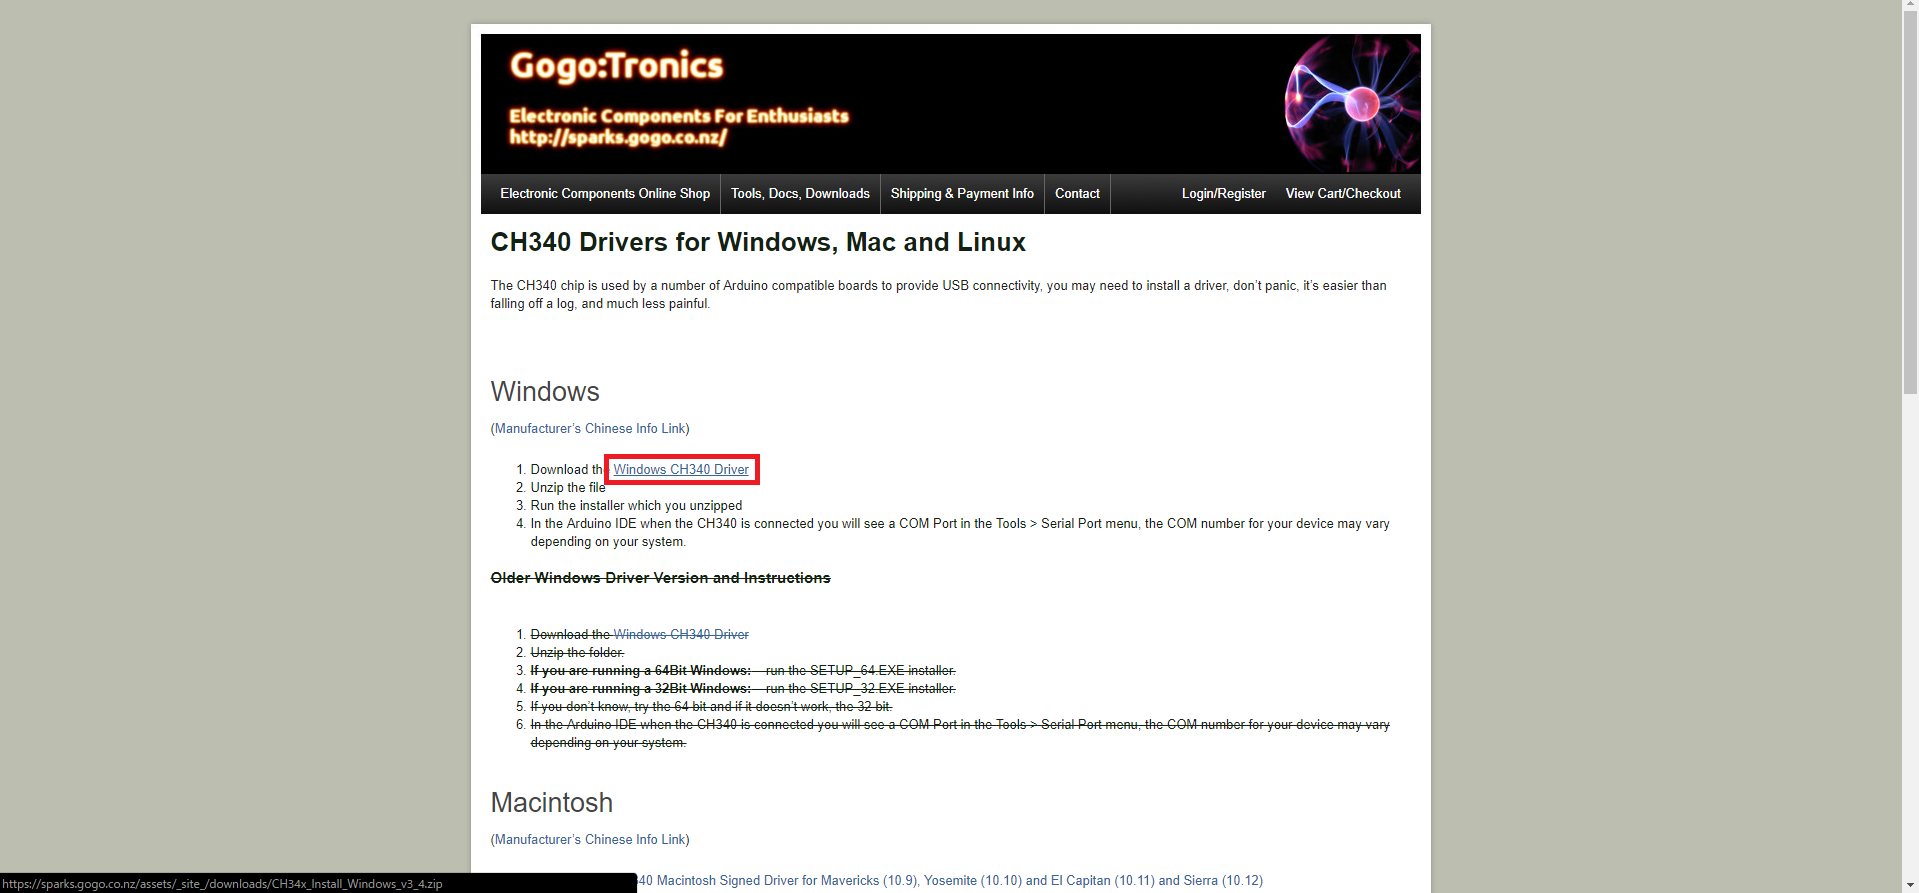
\includegraphics[width=13cm]{driver_2.png}
    \caption{「Windows CH340 Driver」を選択し、ドライバをダウンロードする}
\end{figure}

3.ダウンロードしたファイルはZIPで圧縮されているため、解凍後、
「CH430 Install Windows v3 4.EXE」を実行する。
\begin{figure}
    \centering
    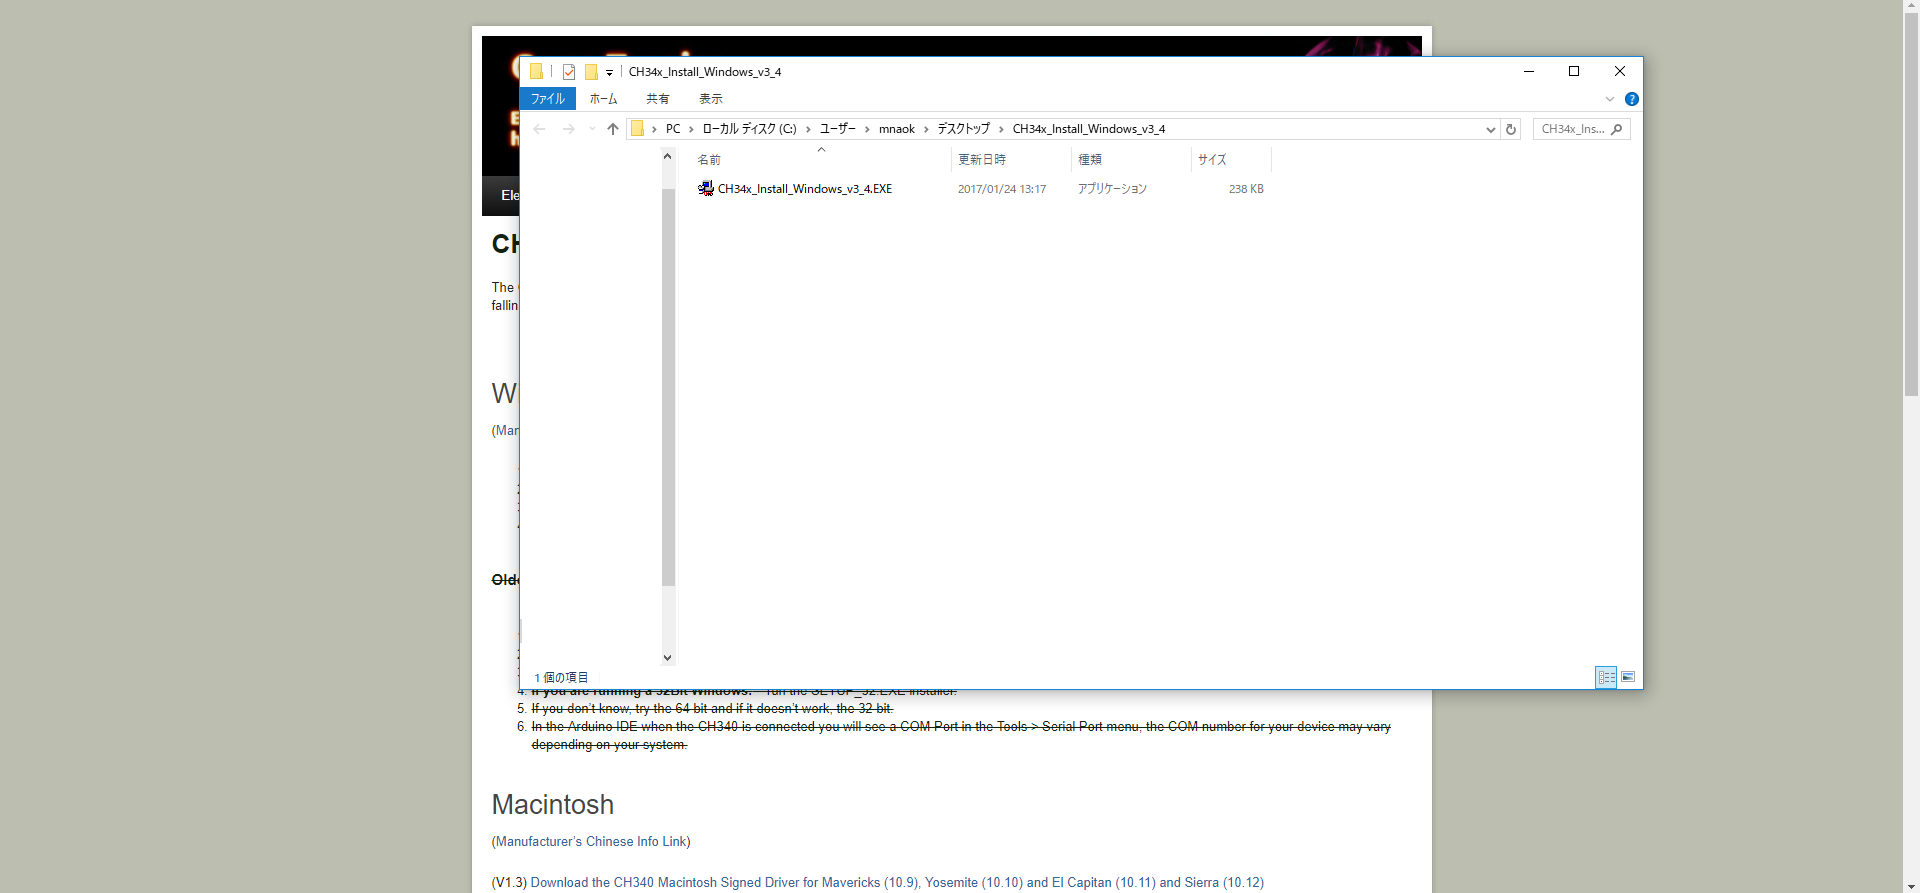
\includegraphics[width=13cm]{driver_3.png}
    \caption{解凍後、「CH340 Install Windows v3 4.EXE」を実行する}
\end{figure}

4.管理者権限を許可すると図のようなウィンドウが現れる。ここで「INSTALL」ボタンを選択する。
\begin{figure}
    \centering
    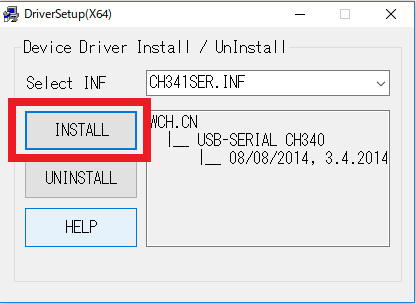
\includegraphics[width=13cm]{driver_4.png}
    \caption{「INSTALL」ボタンを選択する}
\end{figure}

5.成功したような雰囲気のするダイアログが出ればインストールは完了である。
\begin{figure}
    \centering
    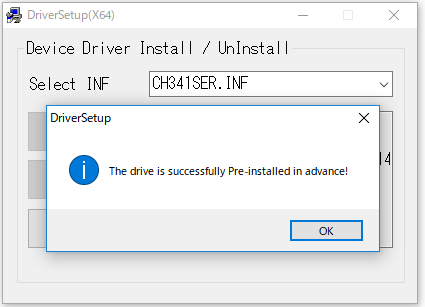
\includegraphics[width=13cm]{driver_5.png}
    \caption{いい感じのダイアログ}
\end{figure}
\clearpage
\subsection{Arduino IDE(統合開発環境)のインストール}
次に、Arduino IDEというArduino専用の開発環境をインストールする。

Vimなどのエディタでも開発することは出来るが難易度の問題上、今回は割愛する。

1.「Arduino IDE」と検索し、「Arduino - Software」を選択する。

2.「Windows Installer, for Windows XP and up」を選択する。

3.「JUST DOWNLOAD」を選択する。寄付をしたい人はしてもよいが、今回は割愛する。

4.ダウンロードした実行形式ファイルを実行する。利用規約をしっかり読み、承諾できるならば「I Agree」を選択する。

5.デフォルトのままで「Next」を選択する。

6.パスの設定をする。デフォルトのままで良いが、変えたい人は変えても良い。「Install」を選択する。

7.インストールが始まる。

8.完了すれば「Completed」と表示される。「Close」を選択し、インストーラーを終了する。
\begin{figure}
    \centering
    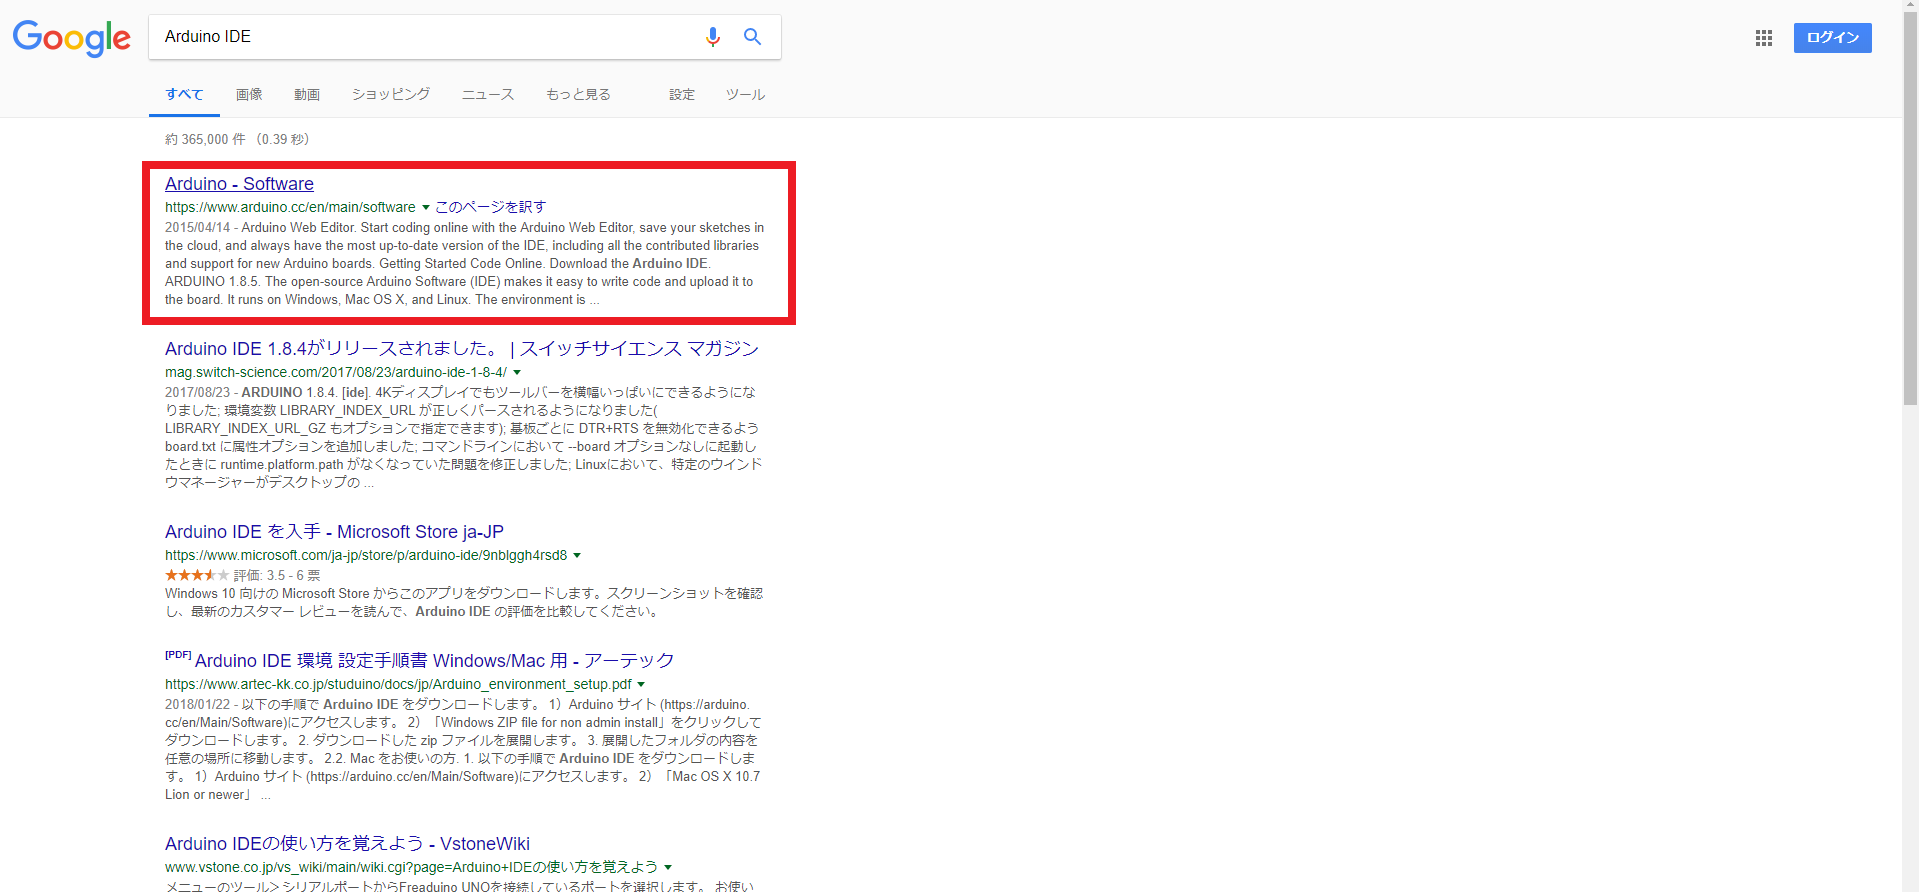
\includegraphics[width=13cm]{found_arduino}
    \caption{「Arduino IDE」と検索し、「Arduino - Software」を選択する}
\end{figure}
\begin{figure}
    \centering
    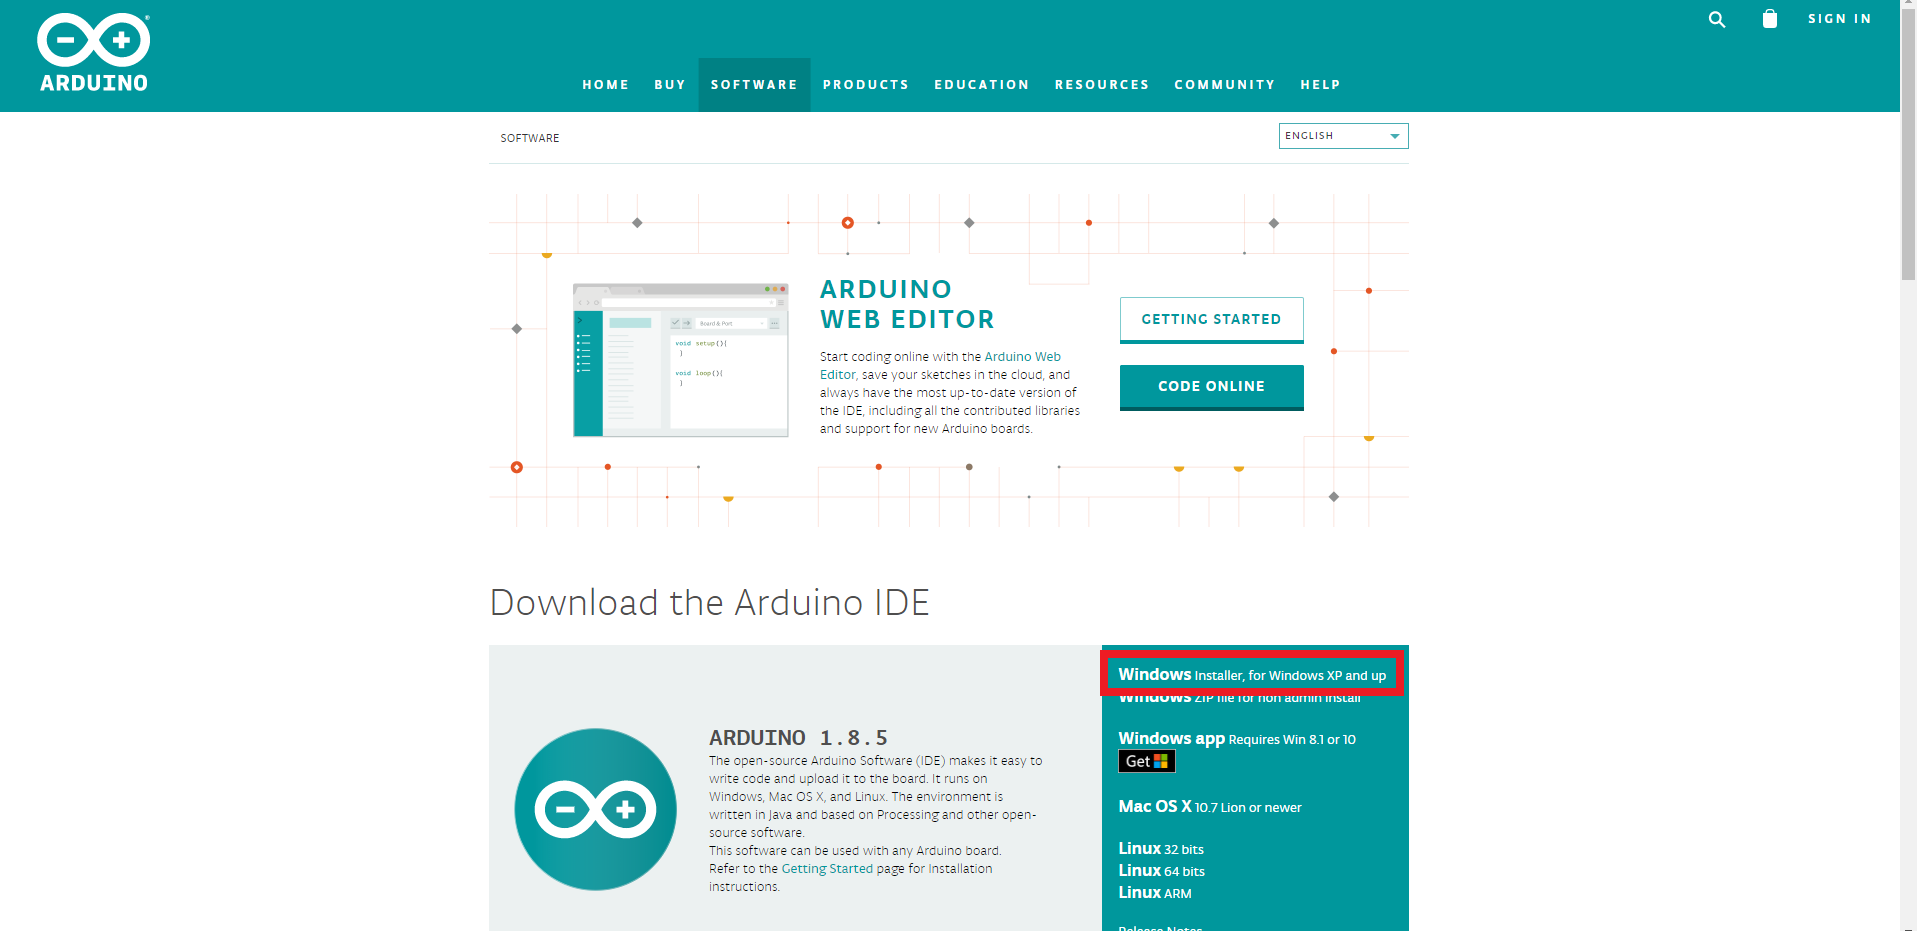
\includegraphics[width=13cm]{download_1.png}
    \caption{「Windows Installer, for Windows XP and up」を選択する}
\end{figure}
\begin{figure}
    \centering
    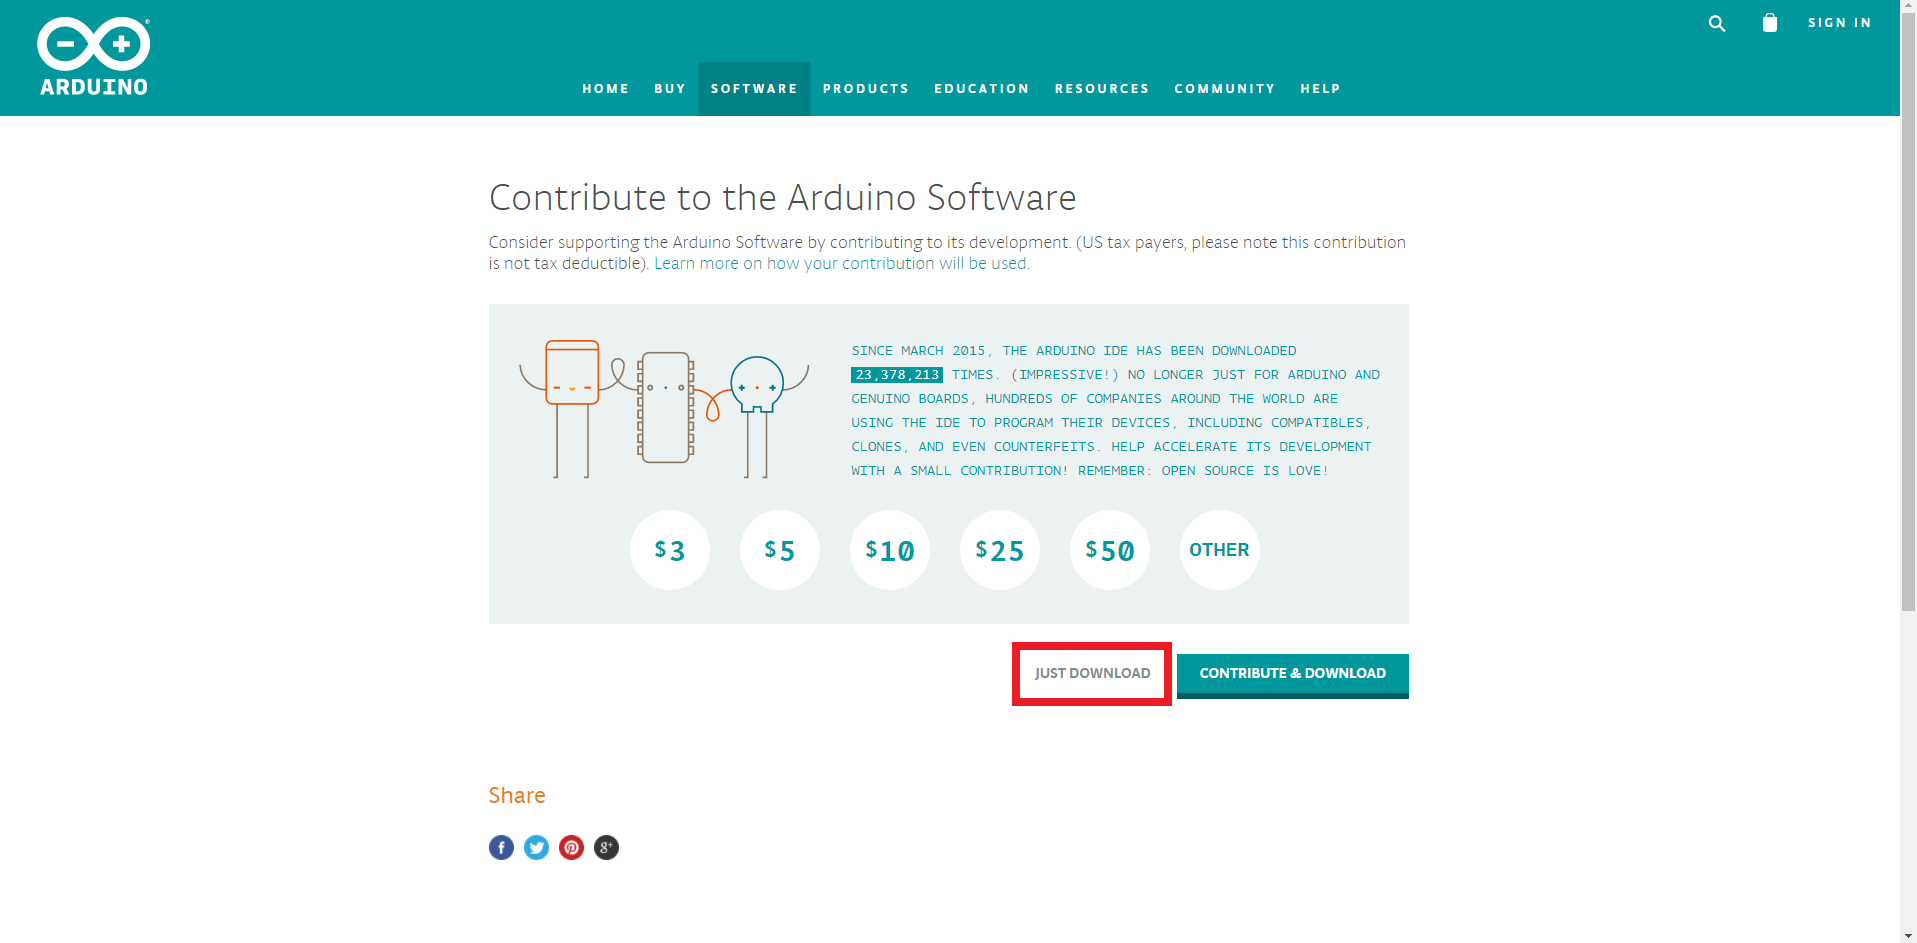
\includegraphics[width=13cm]{download_2.png}
    \caption{「JUST DOWNLOAD」を選択する}
\end{figure}
\begin{figure}
    \centering
    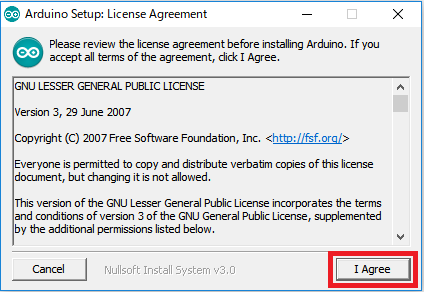
\includegraphics[width=13cm]{arduino_1.png}
    \caption{利用規約をしっかり読み、承諾できるならば「I Agree」を選択する}
\end{figure}
\begin{figure}
    \centering
    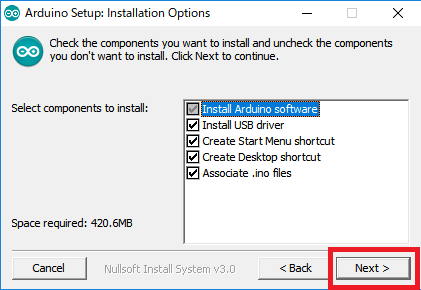
\includegraphics[width=13cm]{arduino_2.png}
    \caption{デフォルトのままで「Next」を選択する}
\end{figure}
\begin{figure}
    \centering
    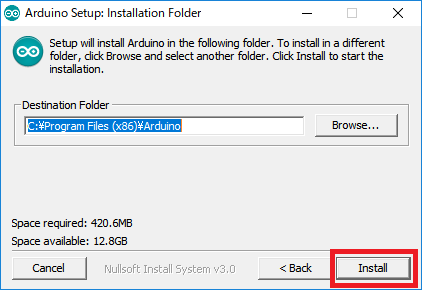
\includegraphics[width=13cm]{arduino_3.png}
    \caption{パスの設定をし、「Install」を選択する。}
\end{figure}
\begin{figure}
    \centering
    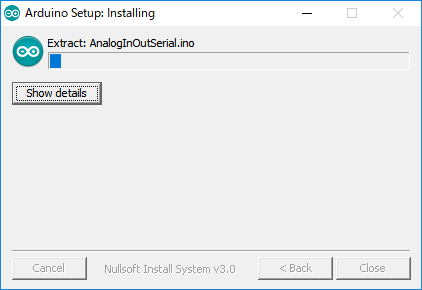
\includegraphics[width=13cm]{arduino_4.png}
    \caption{インストールが始まる。}
\end{figure}
\begin{figure}
    \centering
    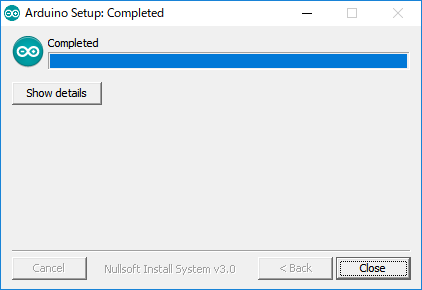
\includegraphics[width=13cm]{arduino_5.png}
    \caption{完了すれば「Completed」と表示される。「Close」を選択し、インストーラーを終了する}
\end{figure}

\clearpage
\section{Arduino IDEについて}
\subsection{使い方}
では、実際にパソコンにマイコンボードを接続し、Arduino IDEを起動してみよう。起動すると以下のような画面が表示される。
\begin{figure}[htbp]
    \centering
    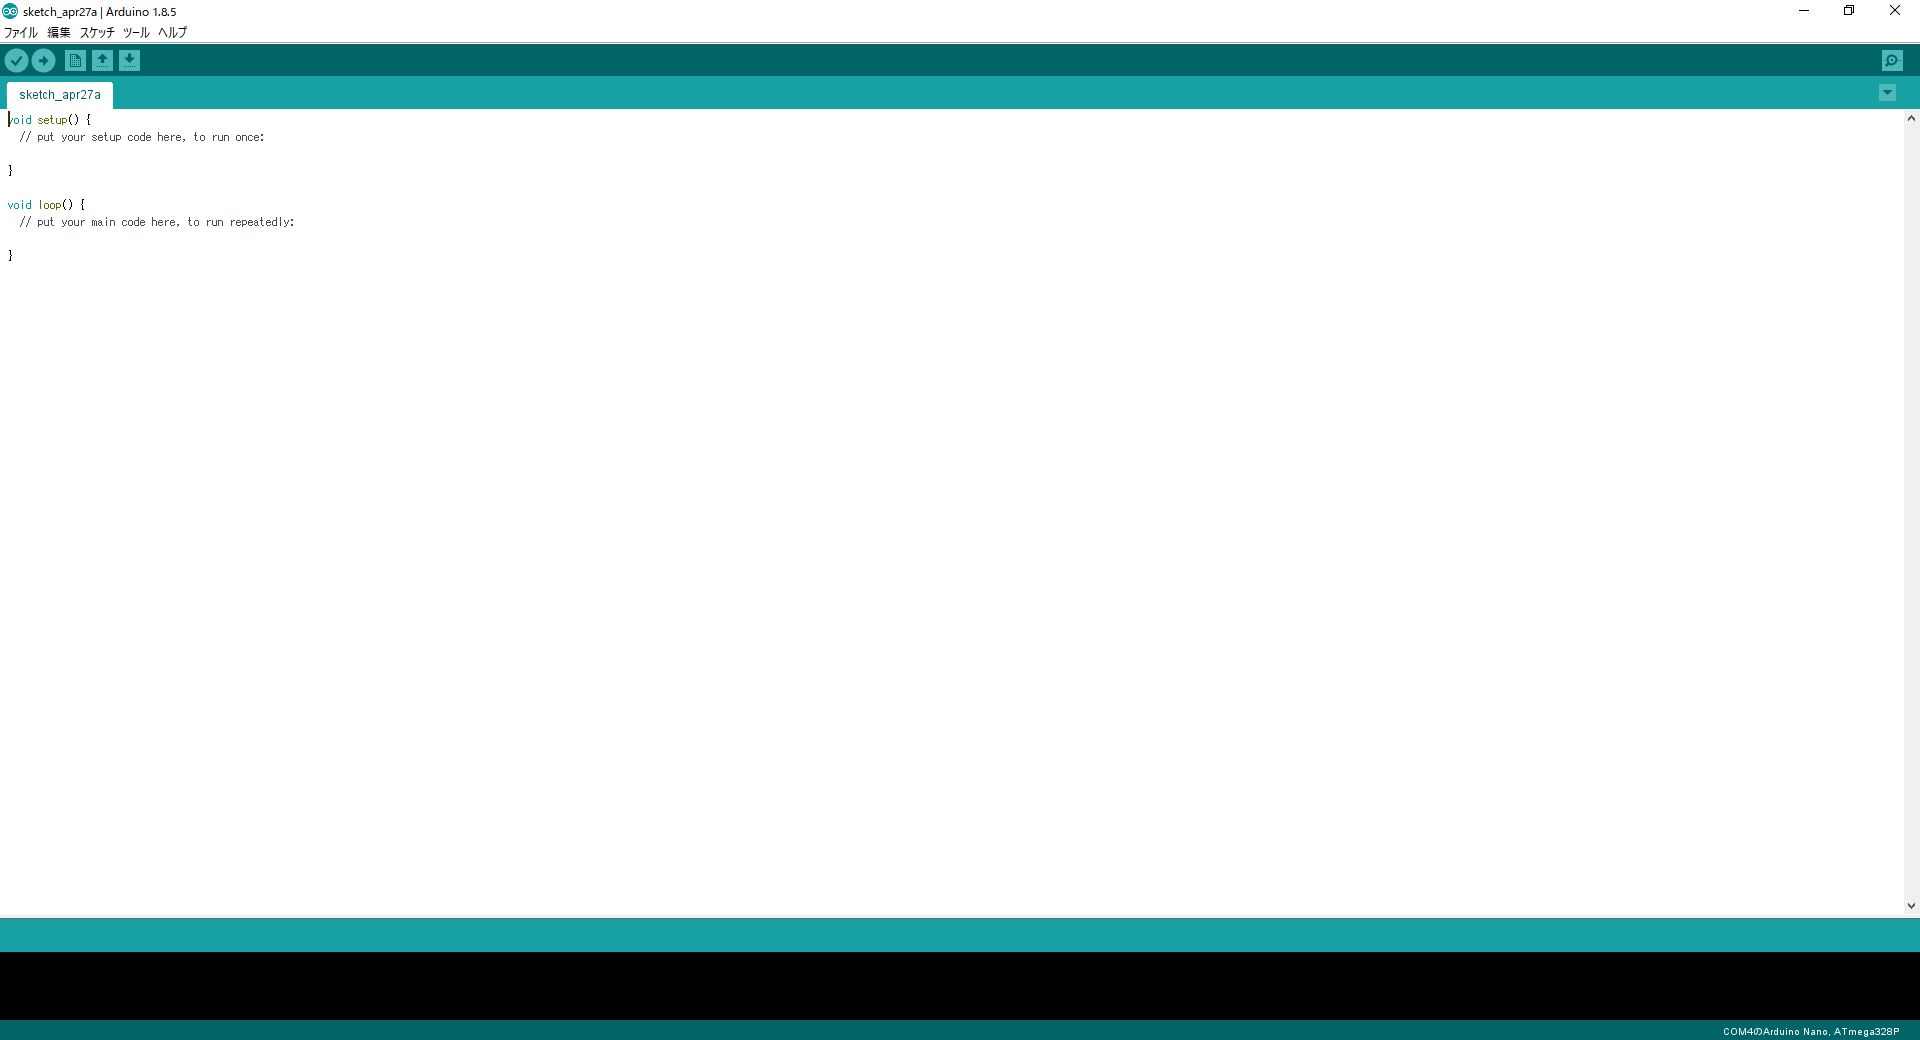
\includegraphics[width=15cm]{ide.png}
    \caption{Arduino IDE}
\end{figure}

画面の大部分を占める白い部分はエディタ領域である。ここにプログラムのソースコードを書いていく。
下部の黒い部分はログビューである。Arduino IDEが実行した作業に関するログ(結果)が表示される。

\begin{figure}[htbp]
    \centering
    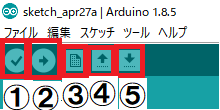
\includegraphics[width=13cm]{ide_button.png}
    \caption{ボタン類}
\end{figure}

左上のボタンについて説明する。

①は「コンパイル実行」ボタンである。
コンパイルとはプログラムをマイコンで実行可能な形式に変換することである。
プログラムの文法に誤りがある場合は、コンパイルが失敗し、誤り箇所をログビューに表示してくれる。

②は「マイコンへの書き込み」ボタンである。
プログラムをコンパイルし、マイコンボードへの書き込みまで一括で行ってくれる。

③は「新規作成」ボタンである。
新たにウィンドウが表示され、別のプログラムを書くことが出来る。

④は「開く」ボタンである。
既存のソースコード(プログラムを記したファイルのことである)を開き、編集することが出来る。

⑤は「保存」ボタンである。
現在編集しているソースコードを保存する。
なお、コンパイル時、もしくは、マイコンへの書き込み時にソースコードは自動で保存される。

\subsection{マイコンボードの設定}
Arduino IDE起動時にはマイコンボードの書き込み設定を行う必要がある。
設定は以下の手順で行う。

1.シリアルポートの設定を行う。上部メニューバーから「ツール」→「シリアルポート」とたどり、「COM X」(Xは数字)を選択する。
ここに現れていない場合は、マイコンが正常に認識されていない。
マイコンボードの電源がついているか、ドライバをインストールしたか確認する必要がある。
よくわからない人は暇そうな先輩に聞くこと。
\begin{figure}[htbp]
    \centering
    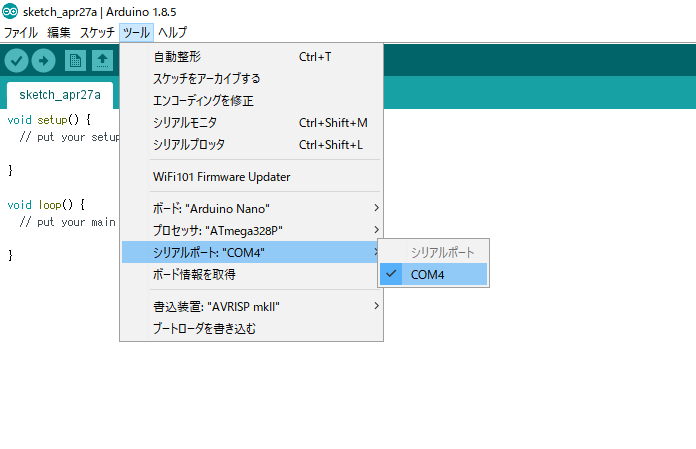
\includegraphics[width=13cm]{serial_config.png}
    \caption{シリアルポートの設定}
\end{figure}

2.マイコンボードの種類を設定する。
上部メニューバーから「ツール」→「ボード」とたどり、「Arduino Nano」を選択する。
\begin{figure}[htbp]
    \centering
    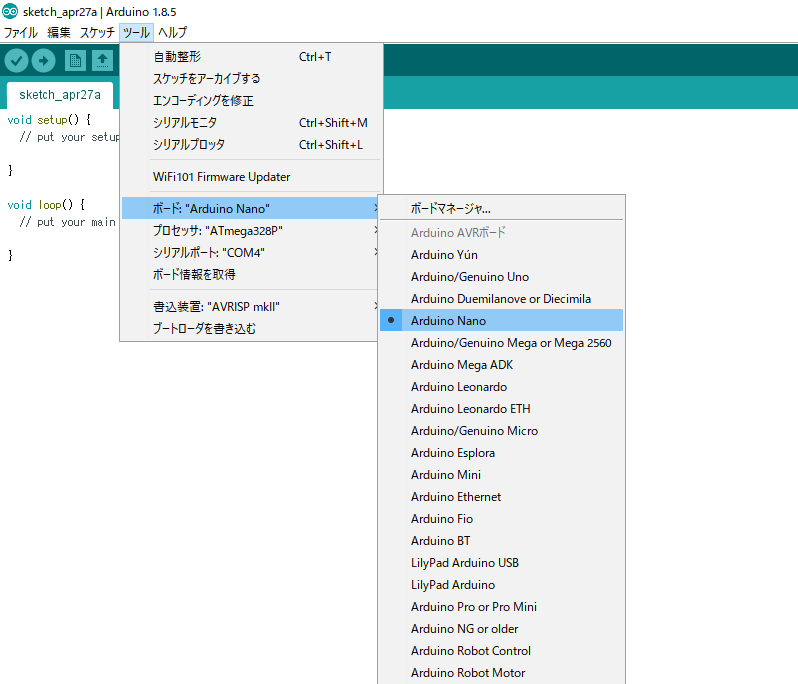
\includegraphics[width=13cm]{board_config.png}
    \caption{ボードの種類の設定}
\end{figure}

\section{C言語について}
本講習はプログラミングを全くしたことがない人を対象にしているが、
C言語について教えるとなると時間も労力もかなり必要になるためArduino C特有の部分のみを重点的に説明している。
C言語について学びたい人は「苦しんで覚えるC言語」(\url{https://9cguide.appspot.com/})や
「やさしいC」(高橋麻奈 著)を読むと良いだろう。
\clearpage
\section{Arduino Cプログラミング}
習うより慣れろということで、実際にプログラミングをしよう。
なお、「Arduino日本語リファレンス」(\url{http://www.musashinodenpa.com/arduino/ref/})を読みながら進めることを強く推奨する。
\subsection{Lチカ(LEDチカチカ)}
\begin{figure}[htbp]
    \centering
    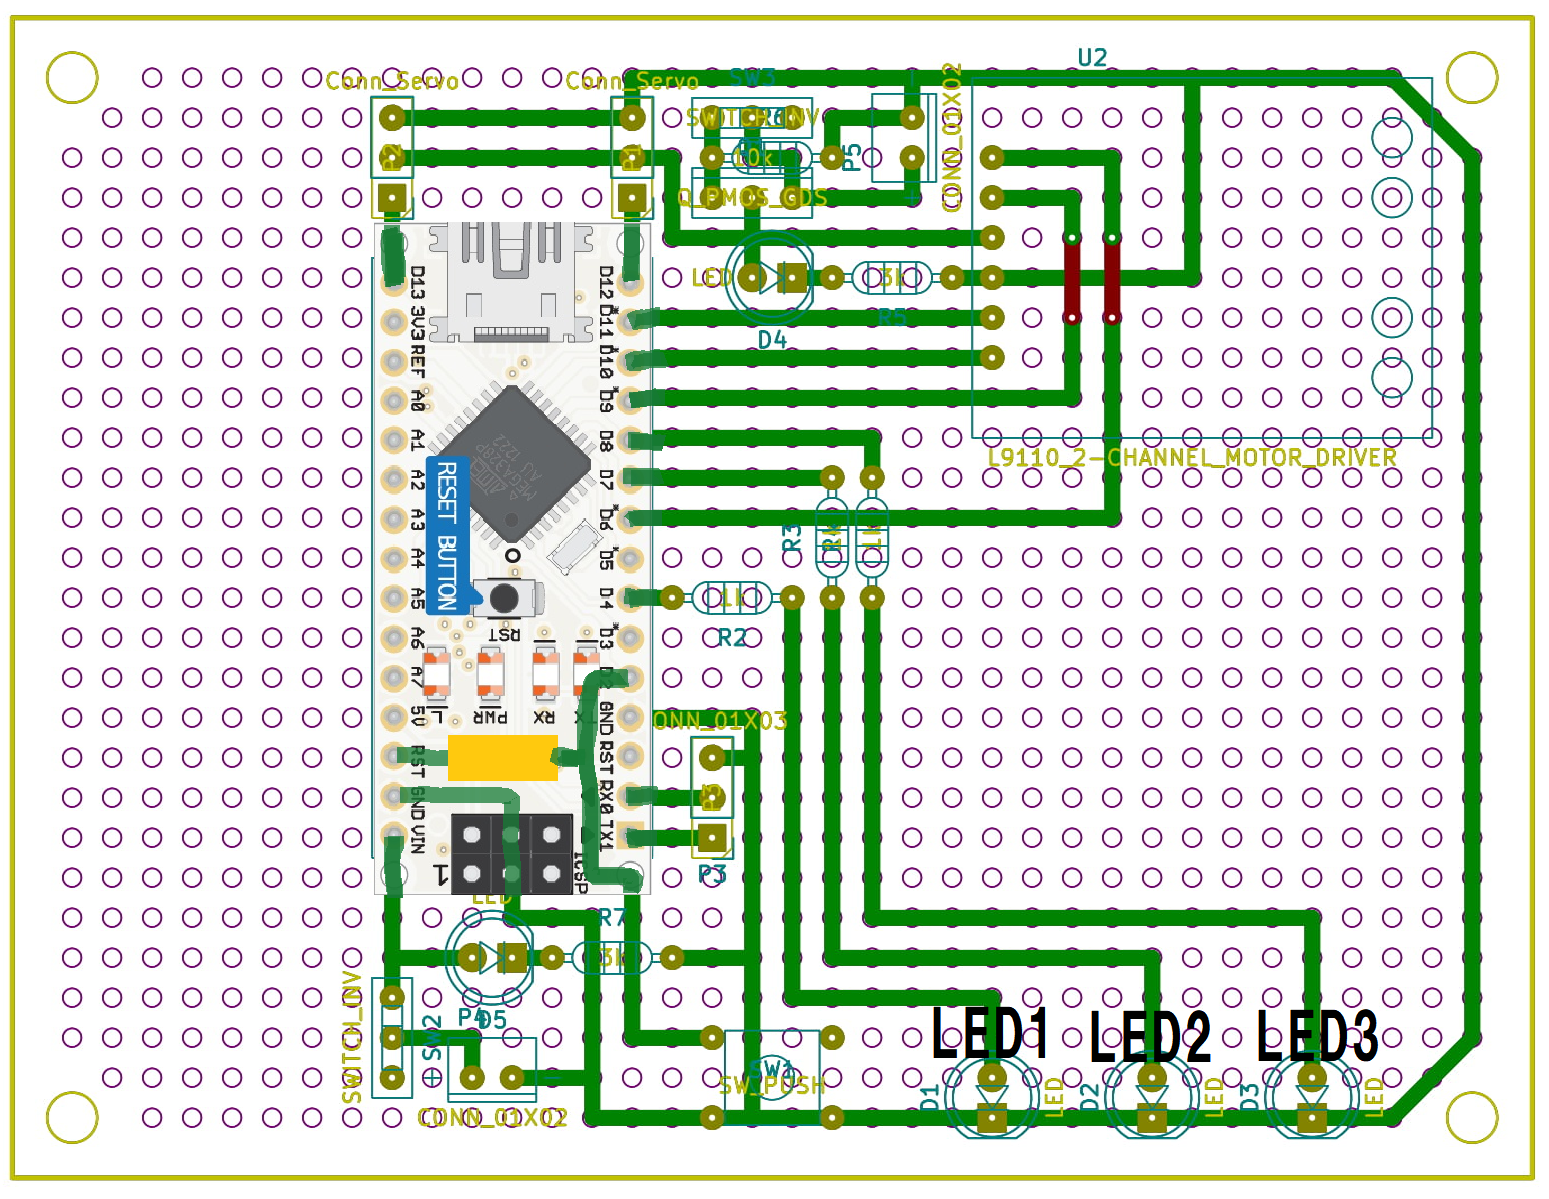
\includegraphics[width=15cm]{l_chika_1.png}
    \caption{Arduino NanoとLEDの接続状態}
\end{figure}
LEDとArduino Nanoの接続状況は上図のとおりである。
LED1はD4ピン、LED2はD7ピン、LED3はD8ピンに接続されている。

次に回路図のLED部分を見てみよう。
\begin{figure}[htbp]
    \centering
    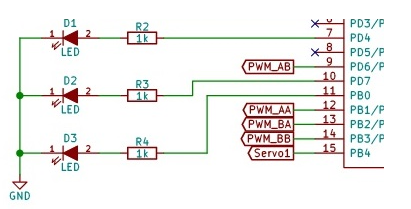
\includegraphics[width=15cm]{l_chika_2.png}
    \caption{回路図上のArduino NanoとLED接続部分}
\end{figure}
LEDのカソードはGNDに接続されている。このときLEDを点灯させるにはどうすれば良いだろうか?
はんだ付け講習でLEDはダイオードであり一方向にしか電流を流さないことを学んだはずである。
アノード側に+を、カソード側にー(GND)をつなげれば、点灯したはずだ。
つまり、$(アノード側の電位)-(カソード側の電位)\geq(LEDの順方向電圧)$となればLEDは点灯する。
詳細な内容は別途、松本以外の誰かが説明してくれるはずである。

要するに、マイコンボード側からLEDに十分な電位をかけてやればいいわけである。
そのために利用するのがデジタルI/Oピンである。

\subsubsection{DigitalPinについて}
DigitalPinは主に、pinを5Vの電源やGNDへ接続
もしくはピンに対して5V、0Vのどちらの電圧がかかっているのか知ることが出来るI/Oピンである。
今回は5Vを出力するために利用する。

\subsubsection{プログラム}
それでは、以下のプログラムを書き写してみよう。
\begin{lstlisting}[basicstyle=\ttfamily\footnotesize, frame=single,caption=Lチカプログラム]
#define LED1 4
#define LED2 7
#define LED3 8
    
void setup() {
    pinMode(LED1, OUTPUT);
    pinMode(LED2, OUTPUT);
    pinMode(LED3, OUTPUT);
}
    
void loop() {
    digitalWrite(LED1, HIGH);
    digitalWrite(LED2, HIGH);
    digitalWrite(LED3, HIGH);
    delay(1000);
    digitalWrite(LED1, LOW);
    digitalWrite(LED2, LOW);
    digitalWrite(LED3, LOW);
    delay(1000);
}    
\end{lstlisting}
書き写せたら、マイコンボードに書き込んでみよう。
エラーなく書き込むことができ、3つのLEDが全て点灯しているだろうか?
問題ないならば、実際にプログラムがどのようになっているのか見ていこう。
\subsubsection{;(セミコロン)について}
;(セミコロン)はC言語における、重要な記号である。実行する関数や式の末尾につけることで、
「この関数(式)はここで終わり」という表現になる。
関数とは実行する操作の書かれた1つのまとまりのことである。
付け忘れると、複数行が1つの関数もしくは式として解釈され、
コンパイルエラーになる。
コンパイルエラーが出る場合はまず、セミコロンを確認しよう。
\subsubsection{\#defineについて}
\#defineとはマクロと呼ばれ、端的に言うと、「定義」である。
つまり、マクロ名と定義した値や式は同一のものとして扱われるわけである。
コンパイル時にマクロ名の部分は定義したものに全て置き換えられる。
つまり、
\begin{lstlisting}[basicstyle=\ttfamily\footnotesize, frame=single]
#define N 10
p = N + N
\end{lstlisting}
は
\begin{lstlisting}[basicstyle=\ttfamily\footnotesize, frame=single]
p = 10 + 10
\end{lstlisting}
と等しいものである。
使うときは
\begin{lstlisting}[basicstyle=\ttfamily\footnotesize, frame=single]
#define マクロ名 定数や式、文字など
\end{lstlisting}
のようにして使う。
\subsubsection{void setup()\{\}について}
void setup()\{\}とは、マイコン起動時に1度だけ実行される関数である。
使うときは
\begin{lstlisting}[basicstyle=\ttfamily\footnotesize, frame=single]
void setup(){
    (Write code here you want to execute)
}
\end{lstlisting}
のようにする。
\subsubsection{void loop()\{\}について}
void loop()\{\}とは、setup()関数が実行された後に、恒久的に実行され続ける関数である。
今回のプログラムでは、LEDの点灯と消灯が無限ループしている。
使うときは
\begin{lstlisting}[basicstyle=\ttfamily\footnotesize, frame=single]
void loop(){
    (Write code here you want to execute)
}
\end{lstlisting}
のようにする。
\subsubsection{pinMode()について}
pinMode()関数は、マイコン起動時に1度だけ実行されている。
この関数は、digitalPinのモードを決定するものであり、
digitalPinのモードとしては
\begin{itemize}
    \item INPUT
    \item OUTPUT
\end{itemize}
がある。

INPUTはdigitalRead()関数と組み合わせて使われることが多い。これに関しては後述する。

OUTPUTは出力するモードであり、digitalWrite()関数と組み合わせて使う。
使うときはpinNumber(ピン番号)とModeを指定し、
\begin{lstlisting}[basicstyle=\ttfamily\footnotesize, frame=single]
void setup(){
    pinMode(pinNumber,Mode);
}
\end{lstlisting}
のようにする。具体的には、
\begin{lstlisting}[basicstyle=\ttfamily\footnotesize, frame=single]
void setup(){
    pinMode(1,OUTPUT);
}
\end{lstlisting}
とすると、D1ピンを出力モードに設定したことになる。なお、ピン番号はDXのXである。
アナログ入力用のAX(Xは数字)はピン番号としてAXをそのまま指定する。
\subsubsection{digitalWrite()について}
前述のpinMode()関数で出力モードに設定したピンで使うことの出来る関数である。
デジタル出力ピンの出力を決定できる。
なお適切にpinModeを設定すればアナログ入力ピンでも利用可能。
出力できる内容としては、
\begin{itemize}
    \item HIGH (主に5V出力)
    \item LOW (0V、GNDに接続された状態)
\end{itemize}
となっている。
使うときはpinNumber(ピン番号)とModeを指定し、
\begin{lstlisting}[basicstyle=\ttfamily\footnotesize, frame=single]
void loop(){
    digitalWrite(pinNumber,Mode);
}
\end{lstlisting}
のようにする。具体的には、
\begin{lstlisting}[basicstyle=\ttfamily\footnotesize, frame=single]
void loop(){
    pinMode(1,HIGH);
}
\end{lstlisting}
とすることで、D1ピンに5Vが出力された状態となる。
\subsubsection{delay()について}
delay()関数は「何もせずに待機」する関数である。
使うときは時間wait\_time (ms単位)を指定し、
\begin{lstlisting}[basicstyle=\ttfamily\footnotesize, frame=single]
delay(wait_time);
\end{lstlisting}
のようにする。具体的には、
\begin{lstlisting}[basicstyle=\ttfamily\footnotesize, frame=single]
delay(100);
\end{lstlisting}
とすることで、100ms待機、つまり0.1秒待機することになる。
\subsubsection{練習問題}
LED1からLED3へと順番に点灯し、LED3からLED1へと順番に消灯するプログラムを書こう!
\clearpage
\subsection{スイッチ入力}
\begin{figure}[htbp]
    \centering
    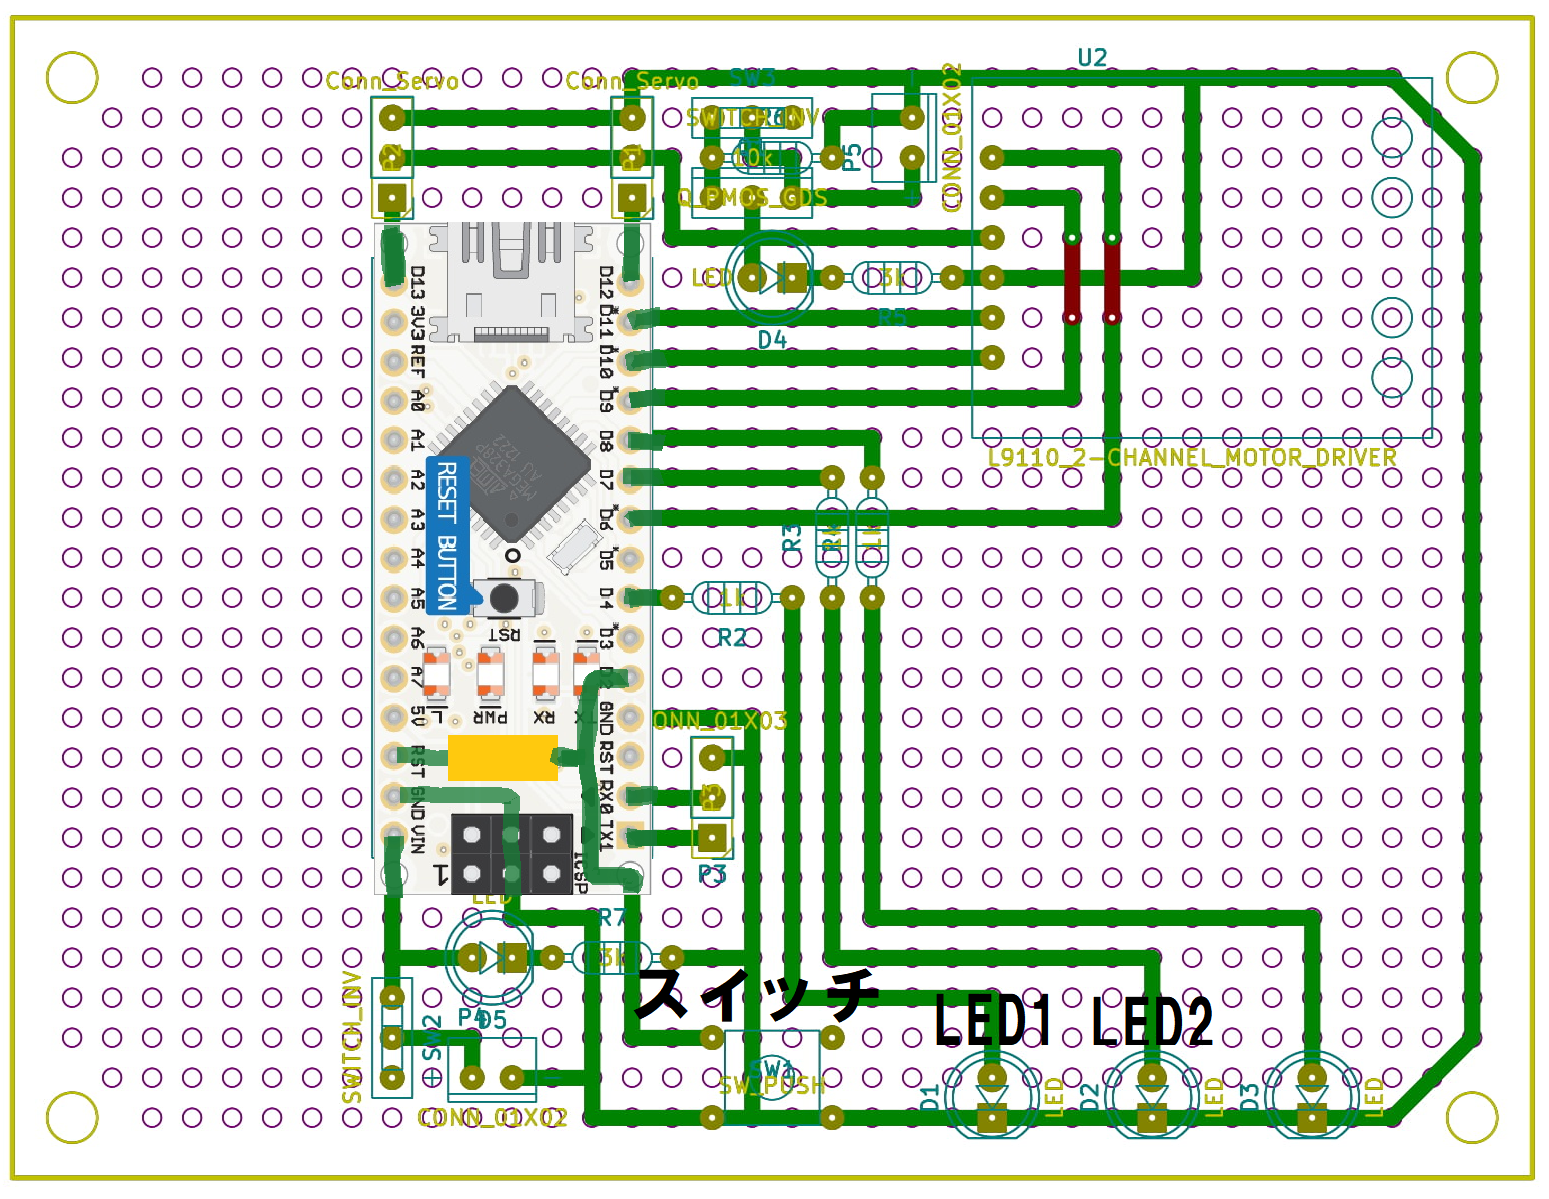
\includegraphics[width=15cm]{switch_1.png}
    \caption{Arduino nano とスイッチの接続状態}
\end{figure}
プッシュスイッチはD2ピン、LED1はD4ピン、LED2はD7ピンに接続されている。

次に回路図のスイッチとLED部分を見てみよう。
\begin{figure}[htbp]
    \centering
    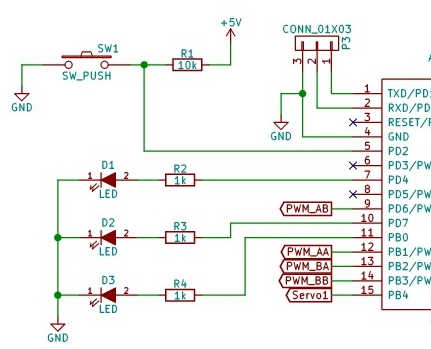
\includegraphics[width=15cm]{switch_2.png}
    \caption{回路図上のArduino nano とスイッチの接続状態}
\end{figure}
ここで重要なのが、スイッチに直列に入った抵抗器R1である。
この状況で使われる抵抗器はプルアップ抵抗と呼ばれ、マイコンの誤作動を抑制するためのものである。

その原理を見ていこう。

まず、プルアップ抵抗がない場合でスイッチがOFFの状態を考える。
\begin{figure}[htbp]
    \centering
    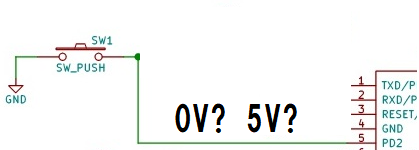
\includegraphics[width=12cm]{switch_5.png}
    \caption{プルアップ抵抗がない状態でのスイッチOFF}
\end{figure}
図のようにD1ピンには何も接続されていない状態となり、0Vでも5Vでもない状態となる。
これはマイコン的には非常にまずい状態であり、ONともOFFとも認識されてしまう状況である。
つまり、誤作動が起きやすい状態なのである。(厳密な原理としてはマイコンのインピーダンスの高さが原因であるが、今回は割愛する。)

そこで、プルアップ抵抗を挿入してみる。
\begin{figure}[htbp]
    \centering
    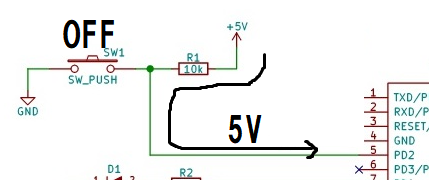
\includegraphics[width=12cm]{switch_3.png}
    \caption{プルアップ抵抗がある状態でのスイッチOFF}
\end{figure}
図を見れば分かるように、スイッチがOFFの状態ではD1ピンに抵抗R1からの5V(厳密には5Vより少し低い)がかけられた状態になり、
マイコンが正常に状態を認識することが出来る。

スイッチがONになった場合は図のようになる。
\begin{figure}[htbp]
    \centering
    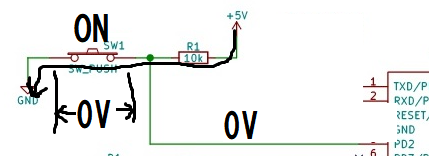
\includegraphics[width=12cm]{switch_4.png}
    \caption{プルアップ抵抗がある状態でのスイッチON}
\end{figure}
スイッチが短絡し、D1ピンはGNDに繋がった状態になるため、マイコンがD1ピンは0Vであると認識することが出来る。
\subsubsection{プログラム}
それでは、また以下のプログラムを書き写してマイコンに書き込んでみよう。
\begin{lstlisting}[basicstyle=\ttfamily\footnotesize, frame=single]
#define LED1 4
#define LED2 7
#define SW 2
    
void setup() {
    pinMode(LED1, OUTPUT);
    pinMode(LED2, OUTPUT);
    pinMode(SW, INPUT);
}
    
void loop() {
    if(digitalRead(SW) == 1){
        digitalWrite(LED1,HIGH);
        digitalWrite(LED2,LOW);
    }else{
        digitalWrite(LED1,LOW);
        digitalWrite(LED2,HIGH);
    }
}
\end{lstlisting}
正常に書き込みができたら動作を確認してみよう。
プッシュスイッチを押していない状態ではLED1だけが点灯し、押した状態ではLED2だけが点灯するはずだ。
\subsubsection{digitalRead()について}
前述したとおり、digitalRead()関数はpinMode()関数でINPUTモードに設定したデジタルピンで
利用可能である。なお適切にpinModeを設定すればアナログ入力ピンでも利用可能。
digitalRead()関数は読み取ったピンの状態に応じて0もしくは1を戻り値とする。
戻り値とは関数実行後に出力される値のことである。
具体的には、戻り値が1な関数foo()があるとすると、
\begin{lstlisting}[basicstyle=\ttfamily\footnotesize, frame=single]
int p = foo();
\end{lstlisting}
は
\begin{lstlisting}[basicstyle=\ttfamily\footnotesize, frame=single]
int p = 1;
\end{lstlisting}
と等価である。
digitalRead()関数はピン番号をpinNumberとすると、
\begin{lstlisting}[basicstyle=\ttfamily\footnotesize, frame=single]
void loop(){
    int p = digitalRead(pinNumber);
}
\end{lstlisting}
のようにする。具体的には、
\begin{lstlisting}[basicstyle=\ttfamily\footnotesize, frame=single]
void loop(){
    int p = digitalRead(1);
}
\end{lstlisting}
となる。D1ピンに5Vがかかっていれば1が戻り値となり、0Vの場合は0が戻り値となる。
\subsubsection{if($\cdots$)\{$\cdots$\}else\{$\cdots$\}について}
digitalRead()関数で取得した値を利用する方法の1つとしてif文がある。
if文は次のような構造になっている。
\begin{lstlisting}[basicstyle=\ttfamily\footnotesize, frame=single]
if(conditional expression){
    (conditional expression is true,code here is executed)
}else{
    (conditional expression is false,code here is executed)
}
\end{lstlisting}
if文は条件式(conditional expression)が正(true)であれば、
すぐ下の範囲のプログラムが実行され、
偽(false)であれば、
else以下のプログラムが実行される。
条件式に使えるものとしては代表的には以下のものが挙げられる。
\begin{itemize}
    \item \verb|==|  a\verb|==|b(a=bならばtrue)
    \item \verb|!=|  a\verb|!=|b(aとbが等しくなければtrue)
    \item \verb|>|   a\verb|>|b(aよりbが大きければtrue)
    \item \verb|<|   a\verb|<|b(aよりbが小さければtrue)
    \item \verb|<|=  a\verb|<|=b(bがa以上であればtrue)
    \item \verb|>|=  a\verb|>|=b(aがb以上であればtrue)
    \item \verb|&&| (AND) A\verb|&&|B(AとBが両者ともにtrueであればtrue)
    \item \textbar\textbar (OR)  A\textbar\textbar B(AとBの少なくとも一方がtrueであればtrue)
\end{itemize}
具体的には以下の通りである。
\begin{lstlisting}[basicstyle=\ttfamily\footnotesize, frame=single]
1 == 2 => false
4 == 4 => true
1 > 2  => false
1 < 2  => true
1 <= 1 => true
4 >= 5 => false
(1!=2)&&(5>2) => true
(1==3)&&(4<7) => false
(1>=2)||(5>2) => true
(2>2)||(7<2) => true
\end{lstlisting}
\subsubsection{練習問題}
1.スイッチを押して離す度に点灯するLEDが右にずれていくプログラムを書こう!

\clearpage
\subsection{PWM(サーボモータ編)}
\begin{figure}[htbp]
    \centering
    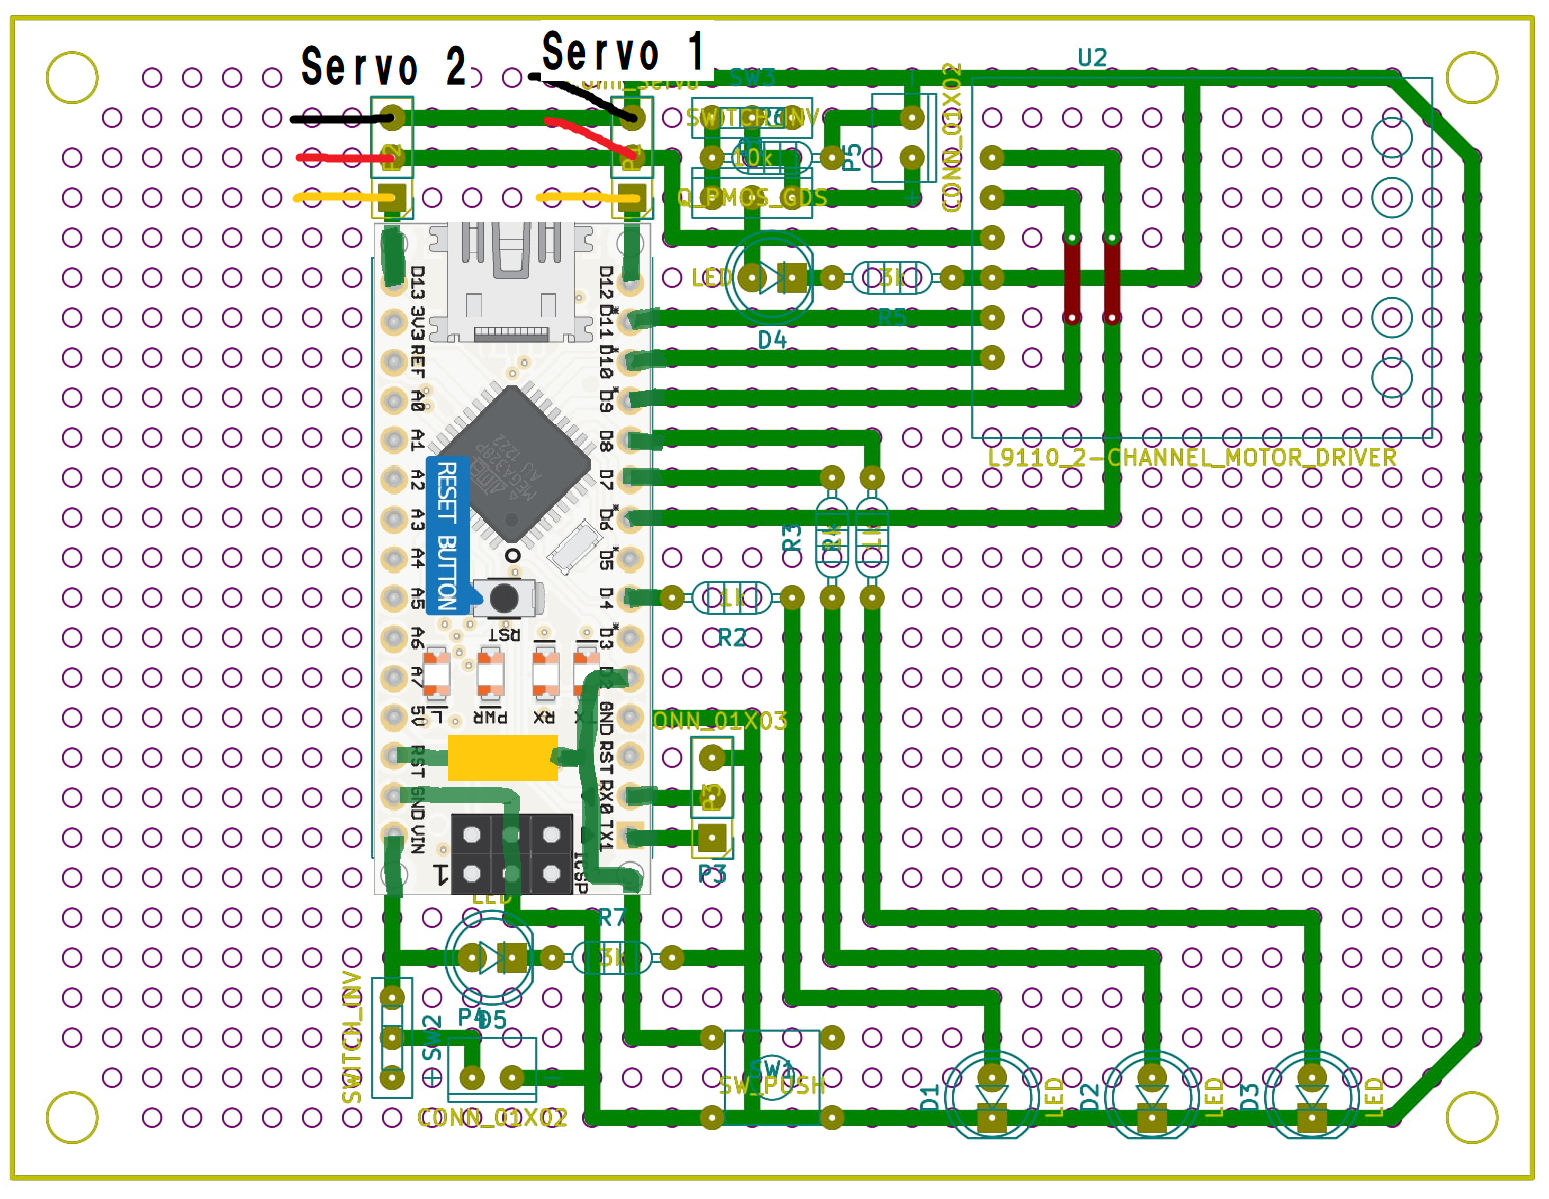
\includegraphics[width=15cm]{servo_pwm.png}
    \caption{サーボモータとArduinoの接続状態}
\end{figure}
サーボモータとArduinoの接続状態は上図のとおりである。
\subsubsection{サーボモータとは}
サーボモータとは、マイコンから与えられた角度に軸を回転させ、保持する部品である。

サーボモータにはいくつかの種類があるが、機械研内で最も利用されているアナログサーボについて説明する。

アナログサーボの制御にはPWMというものが用いられる。
PWMとはONとOFFの比率(Duty比)を変化させながら高速にスイッチングする機能である。
\begin{figure}[htbp]
    \centering
    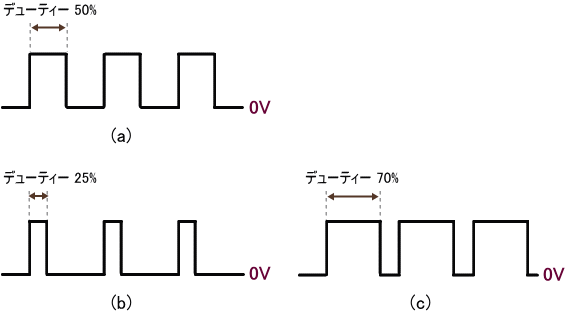
\includegraphics[width=12cm]{pwm_2.png}
    \caption{PWMの波形(http://www.kairo-nyumon.com/pwm\_signal.htmlより)}
\end{figure}
アナログサーボモーターではこのDuty比を変化させることで角度を指定している。
ArduinoではServoオブジェクトを用いることで容易に制御することが出来る。
\subsubsection{プログラム}
それでは、例のごとく以下のプログラムを書き写そう。
\begin{lstlisting}[basicstyle=\ttfamily\footnotesize, frame=single]
#include <Servo.h>
Servo servo1;
Servo servo2;
void setup() {
    servo1.attach(12);
    servo2.attach(13);
}
    
void loop() {
    servo1.write(30);
    servo2.write(30);
    delay(500);
    servo1.write(60);
    servo2.write(60);
    delay(500);
    servo1.write(90);
    servo2.write(90);
    delay(500);
    servo1.write(120);
    servo2.write(120);
    delay(500);
    servo1.write(150);
    servo2.write(150);
    delay(500);   
}
\end{lstlisting}
書き写せたならばマイコンボードに書き込もう。
書き込みが完了するとサーボモーターが少しずつ回転しているはずである。
\subsubsection{\#includeについて}
\#includeとは主にライブラリの読み込み指定に用いられる。ライブラリとは関数やクラスなどをまとめたものである。
サーボモーターを制御するServoクラスでは別途ライブラリを読み込む必要があるため、以下のコードを
プログラムの先頭に挿入する必要がある。
\begin{lstlisting}[basicstyle=\ttfamily\footnotesize, frame=single]
#include <Servo.h>
\end{lstlisting}
\subsubsection{Servoクラスについて}
クラスについて説明するとなると莫大な労力を要するため詳しく知りたい人は
別途自分で調べること。ここでは具体的な利用方法についてのみ説明する。

まず、使いたいサーボの個数分だけServoクラスの変数(インスタンス)を宣言する。
\begin{lstlisting}[basicstyle=\ttfamily\footnotesize, frame=single]
Servo servo1
Servo servo2
\end{lstlisting}
ここでは、サーボを2つ用いるため、servo1とservo2の2つのインスタンスを宣言した。
次に、各インスタンスに制御するピンを割り当てる。
ピンを割り当てるときに使うのがattach()関数である。以下のようにしてピンを割り当てる。
\begin{lstlisting}[basicstyle=\ttfamily\footnotesize, frame=single]
void setup() {
    servo1.attach(12);
    servo2.attach(13);
}
\end{lstlisting}
ここではservo1にD12ピンを、servo2にD13ピンを割り当てている。
ピンの割当ができれば、次はサーボモータの角度を指定する。
このときに使うのがwrite()関数である。
\begin{lstlisting}[basicstyle=\ttfamily\footnotesize, frame=single]
void loop(){}
    servo1.write(30);
    servo2.write(45);
}
\end{lstlisting}
ここでは、servo1に30度、servo2に45度を指定している。
指定可能な角度としては普通のサーボであれば0〜180度である。
\subsubsection{練習問題}
1.スイッチを押す度に角度が10度ずつ増加し、180度まで達した後はスイッチを押す度に10度ずつ減少するプログラムを書こう
\clearpage
\subsection{PWM(モータードライバ編)}
マイコンボード上にあるコネクタがついた基板はモータードライバというもので、
大電流を流さなければならないモーターを駆動するものである。
\subsubsection{モーターの制御におけるPWMについて}
なぜモーターの制御でPWMを使うのか説明しておく。
よく使うDCモーターは電圧に応じて回転速度・トルクが増減する。
しかし、レギュレーターなどで電圧を下げると、
電圧差の分だけが熱となり失われてしまう。
その対策として、ON,OFFの時間比率(Duty比)を制御することで、時間平均すれば電圧を変化させていることと
同等のものとしてみなせるPWMがよく用いられる。
(PWMはモーターのインダクタンスのおかげでうまく動作しているらしいが詳しいことは割愛する)
具体的には図のようにDuty比を変化させることでDCモーターの速度を制御している。
\begin{figure}[htbp]
    \centering
    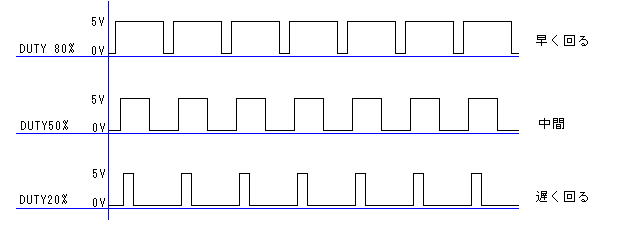
\includegraphics[width=15cm]{pwm.jpg}
    \caption{PWMのDuty比(http://www.hokutodenshi.co.jp/PUPPYSupportPage/ensyu/pwm/pwm1.htmlより)}
\end{figure}
\subsubsection{モータードライバL9110の制御方法}
モータードライバを用いてPWM制御する方法を説明する。
今回用いるモータードライバはL9110というものであり、Googleなどで検索すれば
データシート(部品の仕様書)が見つかる。下に要点のみ抜き出したデータシートの一部を示す。
\begin{figure}[htbp]
    \centering
    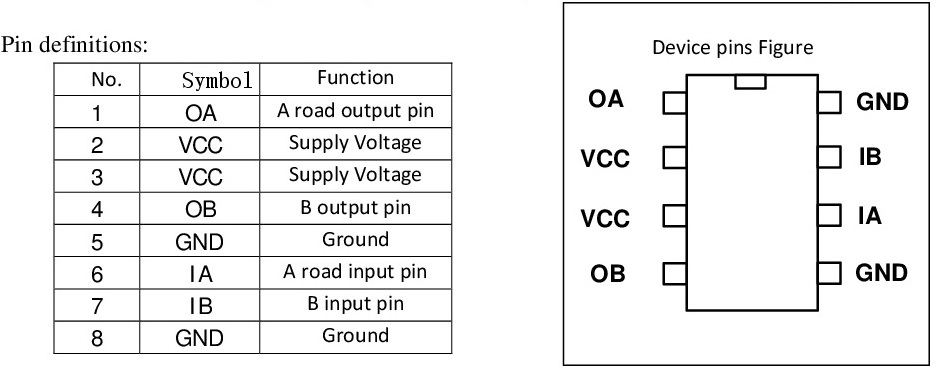
\includegraphics[width=13cm]{datasheet_1.jpg}
    \caption{ICパッケージに関する部分}
\end{figure}
今回はモジュール化された基板を用いるため、ICパッケージに関しては直接気にする必要はない。
しかし、入力が2つあり、出力が2つあることは把握しておく必要がある。
\begin{figure}[htbp]
    \centering
    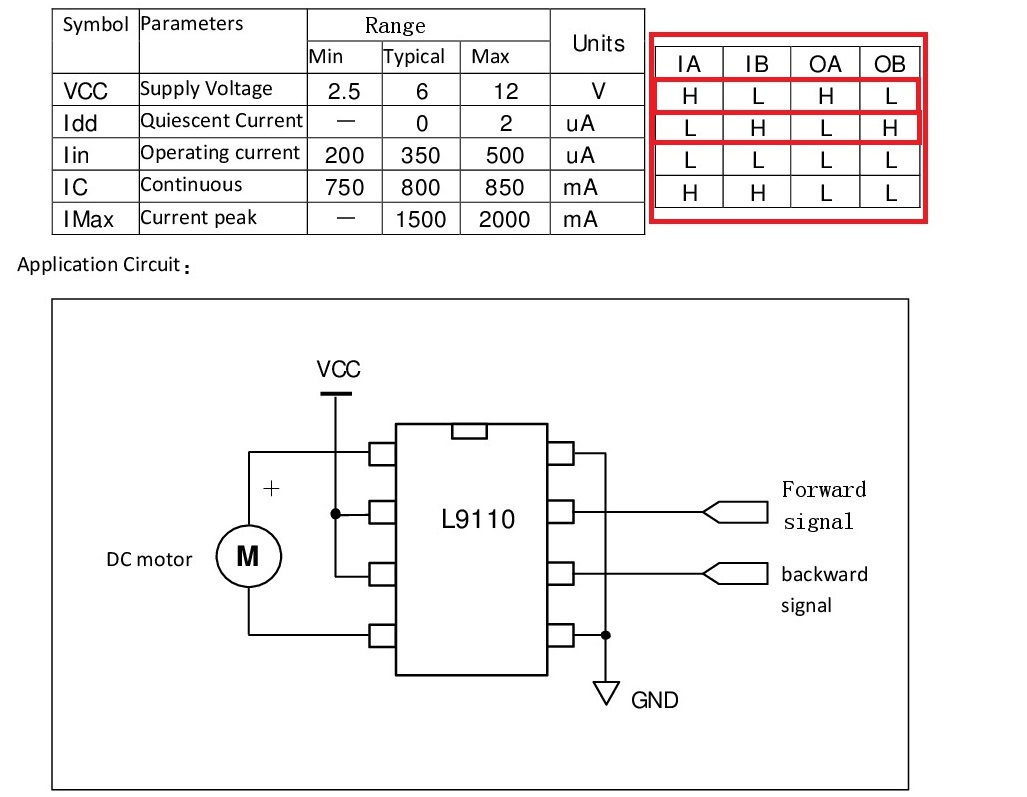
\includegraphics[width=13cm]{datasheet_2.jpg}
    \caption{PWMの入力と出力に関する部分}
\end{figure}
赤い四角で囲まれた表が最も重要である。
ここからIAとIBにかける電圧の組み合わせによって出力端子の様子が変化することが分かる。
ちなみに、Hは電源電圧、Lは0Vである。

それでは組み合わせを詳しく見ていこう。
\begin{itemize}
    \item IAとIBの両者を同じ状態にすると出力は必ずLになっている。
    \item IAをH、IBをLにするとOAがH、OBがLとなる。このときのモーターの回転を正転とする。
    \item IAをL、IBをHにするとOAがL、OBがHとなる。上の場合と考えるとモーターにかかる電位が逆になり、モーターが逆転する。
\end{itemize}
このようになっている。つまり、正転させたい場合はIBを常にLにしておき、IAにPWMを入力すれば良い。
逆転させたいときは、逆にIAを常にLにしておき、IBにPWMを入力すれば良い。
\subsubsection{プログラム}
それでは、例のごとく以下のプログラムを書き写そう。
\begin{lstlisting}[basicstyle=\ttfamily\footnotesize, frame=single]
#define MOTOR_A1 6
#define MOTOR_A2 9
#define MOTOR_B1 10
#define MOTOR_B2 11

void setup() {

}
    
void loop() {
    analogWrite(MOTOR_A1, 100);
    analogWrite(MOTOR_B1, 100);
    analogWrite(MOTOR_A2, 0);
    analogWrite(MOTOR_B2, 0);
    delay(1000);
    analogWrite(MOTOR_A1, 255);
    analogWrite(MOTOR_B1, 255);
    delay(2000);
    analogWrite(MOTOR_A1, 0);
    analogWrite(MOTOR_B1, 0);
    analogWrite(MOTOR_A2, 100);
    analogWrite(MOTOR_B2, 100);
    delay(1000);
    analogWrite(MOTOR_A2, 255);
    analogWrite(MOTOR_B2, 255);
    delay(2000);
}
\end{lstlisting}
うまく書き込めたならば、
モーターが動き出し速度が速くなった後に逆転で動き出し以降同じような動きをする。
\subsubsection{analogWrite()について}
analogWrite()関数はPWM出力のDuty比を指定する関数である。
Duty比は0(0\%)〜255(100\%)で指定することが出来る。
なお、analogWrite()関数はPWM出力が利用可能な端子でのみ利用可能である。
ピン番号をpinNumber、Duty比をdとすると次のようになる。
\begin{lstlisting}[basicstyle=\ttfamily\footnotesize, frame=single]
void loop() {
    analogWrite(pinNumber, d);
}
\end{lstlisting}
具体的には以下のとおりである。
\begin{lstlisting}[basicstyle=\ttfamily\footnotesize, frame=single]
void loop() {
    analogWrite(6, 255);
}
\end{lstlisting}
D6ピンに対してDuty比100\%のPWMを出力することになる。
\subsubsection{練習問題}
1.スイッチを押す度に回転速度が少しずつ早くなり、
最高速度に達した後は少しずつ減少し、
正転から逆転に切り替わり同じように正転時と同じ動作をするプログラムを書こう。
\clearpage
\subsection{シリアル通信}
シリアル通信はマイコンとの通信手段の1つである。
おもにマイコン同士やパソコンとの通信で利用される。
\subsubsection{Arduino IDEのシリアルモニタ}
Arduino IDEにはマイコンとのシリアル通信をするためのシリアルモニタが標準搭載されている。
ポート設定とボード設定を完了した状態で、「ツール」→「シリアルモニタ」と選択すると、
シリアルモニタが起動する。
\begin{figure}[htbp]
    \centering
    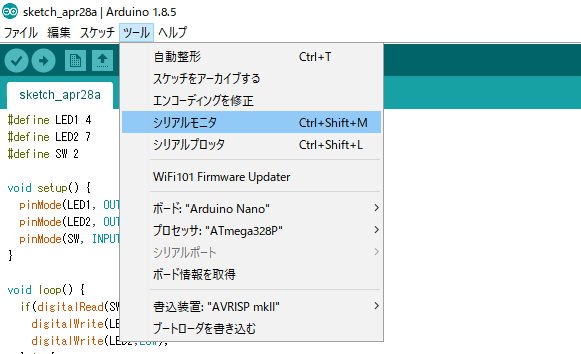
\includegraphics[width=13cm]{serial_1.png}
    \caption{シリアルモニタ起動}
\end{figure}
\subsubsection{プログラム}
それでは、例のごとく以下のプログラムを書き写そう。
\begin{lstlisting}[basicstyle=\ttfamily\footnotesize, frame=single]
void setup()  {
    Serial.begin(9600);
    Serial.println("HelloWorld!");
}
      
void loop() {
    if (Serial.available()>0){
        Serial.write(Serial.read());
    }
}
\end{lstlisting}
\begin{figure}[htbp]
    \centering
    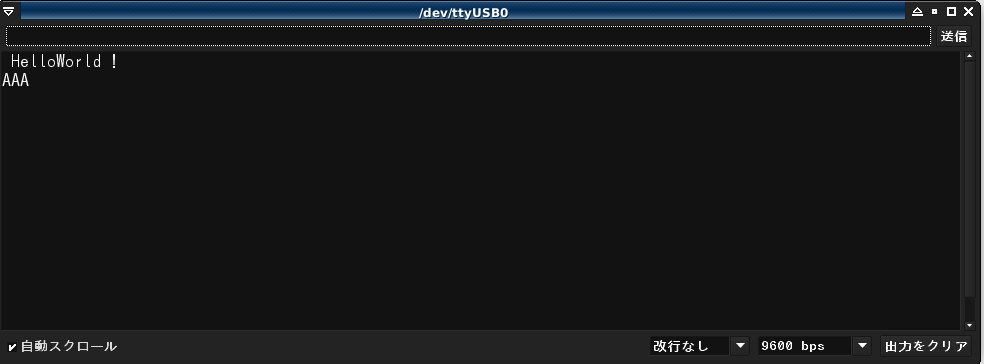
\includegraphics[width=13cm]{serial_3.png}
    \caption{正常に動作している図}
\end{figure}
\subsubsection{Serial.begin()について}
begin()関数はシリアル通信を行う場合必ず実行する必要がある。
引数は通信速度であり、単位はbps(bit per second)である。

ただし、通信可能な速度は限られているため、
特別な場合を除いては9600bpsを指定すること。
\begin{lstlisting}[basicstyle=\ttfamily\footnotesize, frame=single]
void setup() {
    Serial.begin(9600);
}
\end{lstlisting}
\subsubsection{Serial.println()について}
println()関数は文字列をシリアル通信で送信する関数である。
引数は整数型かString型である必要がある。
print()関数との違いは、print()関数は改行しないが、println()関数は改行する点である。
\begin{lstlisting}[basicstyle=\ttfamily\footnotesize, frame=single]
void loop() {
    Serial.println("HOGE");
}
\end{lstlisting}
とすると文字列「HOGE」が送信される。
\subsubsection{Serial.write()について}
write()関数は整数や文字列をバイナリで送信する関数である。
\begin{lstlisting}[basicstyle=\ttfamily\footnotesize, frame=single]
void loop() {
    Serial.write("HOGE");
}
\end{lstlisting}
とすると文字列「HOGE」がバイナリで送信される。
\subsubsection{Serial.avalilable()とSerial.read()について}
\begin{figure}[htbp]
    \centering
    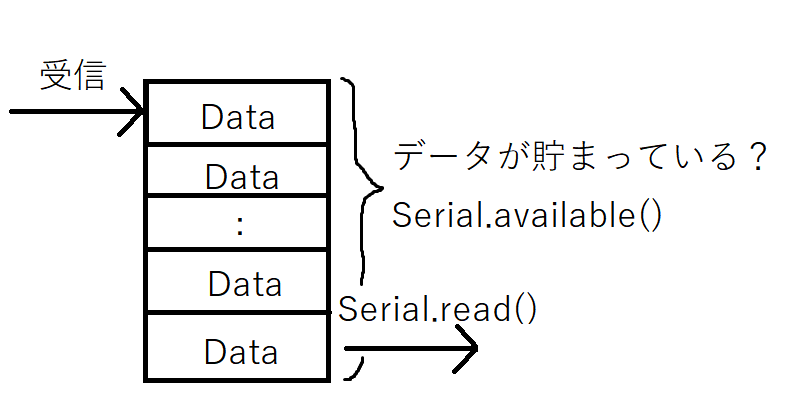
\includegraphics[width=13cm]{serial_2.png}
    \caption{Serial.avalilable()とSerial.read()}
\end{figure}
avalilable()関数とread()関数は図の通りの関係である。

シリアル通信で受信したデータは1byteずつバッファー(データの一時保管場所)に蓄積される。
available()関数はバッファーにデータが存在しているか確認し、存在する場合はその合計byte数を
戻り地として返し、存在しない場合は0を返す。
read()関数はバッファーの一番古いデータから1byteだけ取り出す関数である。
取り出したデータはバッファーから消える。
具体的にはif文やwhile文と組み合わせて使うことが多い。
\begin{lstlisting}[basicstyle=\ttfamily\footnotesize, frame=single]
void loop() {
    String str;
    while(Serial.avalilable() > 0){
        str += Serial.read();
    }
}
\end{lstlisting}
上のようにすると、受信したデータをString型変数strにどんどん代入していくことになる。
\subsubsection{練習問題}
以下の練習問題は「Arduino日本語リファレンス」(\url{http://www.musashinodenpa.com/arduino/ref/})の「Stringクラス」やGoogle検索を利用すること。

(ヒント:Stringクラスには文字列(String型)を数値(Int型)に変換するメソッドが存在する。なお、Arduino日本語リファレンスには記載されていないため、検索すること。)

1.シリアルモニタで送信した値にサーボモーターの角度を変化させるプログラムを書こう

2.シリアルモニタで送信した速さでモーターが回転するプログラムを書こう

\clearpage
\subsection{Advancedな課題}
これまでのプログラミング演習に物足りない人は以下の項目を実践してみるのも良いだろう。
\begin{itemize}
    \item 通信形式がI2Cなセンサの値を読み取りシリアルで出力する。
    \item 通信形式がSPIなセンサの値を読み取りシリアルで出力する。
    \item 一度のシリアル通信で複数の値を送受信する。
    \item Arduinoのレジスタの設定を変更し、ADCの速度を高速化する。
    \item 圧電スピーカーを利用して音楽を演奏する。
    \item センサの値をArduino内で記録し、一定時間ごとにシリアル通信経由でデータを送り、パソコン側は自動でCSVファイルに保存する。
\end{itemize}

\subsection{できれば学習してほしいこと}
以下に自主的な学習を強く推奨する事柄を示す。
\begin{itemize}
    \item GitおよびGitHubによるソースコード管理の習得
\end{itemize}

\section{最後に}
マイコン講習を受け、回路講習で制作した機械研マイコンボードの基本的な機能は使いこなせるようになったはずだ。
部内ロボコンだけでなく、ほかの製作物でもマイコンは必ず使うものであり、
使いこなすことができれば製作可能な範囲はかなり広がる。
機械研マイコンボードを性能不足に感じるようになったならば、STM32などの高性能なマイコンを利用すれば良いだろう。
出来る限り多くのプログラムを書き、試行錯誤してもらいたい。
\end{document}